\chapter{Kiểm định hệ thống và kết quả thực nghiệm}
\label{chap:results}

\section{Thiết kế thực nghiệm và môi trường kiểm định}

Tuân thủ chuẩn mực đánh giá Kỹ thuật phần mềm thực nghiệm~\cite{wohlin2012experimentation}, chương này đánh giá \textbf{CITRA} (\texttt{v3.91.3}) thông qua các bộ kiểm thử tự động (đơn vị, tích hợp, trình duyệt), ma trận truy vết yêu cầu hai chiều và năm câu hỏi nghiên cứu (\textbf{RQ1}--\textbf{RQ5}) kết hợp đo kiểm tầng quyết định có kiểm soát, đánh giá trực tuyến 15 API, kiểm toán từng dòng bản thảo thực tế và kiểm thử chịu tải vận hành.

\subsection{Các câu hỏi nghiên cứu}

\begin{itemize}
    \item \textbf{RQ1 (Độ chính xác tầng quyết định trong phân phối và thực nghiệm loại bỏ thành phần):} Động cơ lai Nơ-ron -- Ký hiệu phân loại chính xác đến mức nào trên tập đo kiểm tách biệt theo bài báo gốc so với các phương pháp cơ sở loại bỏ thành phần (\texttt{B0}--\texttt{B4}) và mô hình Hồi quy Logistic Đa lớp 16 đặc trưng thuần túy (\texttt{B5})?
    \item \textbf{RQ2 (Độ bền vững của rào chắn ký hiệu ngoài phân phối):} Các rào chắn ký hiệu rời rạc thực thi chính sách toàn vẹn không cần huấn luyện lại (bài báo bị rút lại, DOI lai ghép, URL giữ chỗ RFC 2606, DOI khu vực, cạn hạn mức API và sai lệch thẩm quyền luật VN) hiệu quả ra sao khi bộ phân loại tuyến tính liên tục thất bại?
    \item \textbf{RQ3 (Hiệu chỉnh xác suất và độ ổn định thang điểm CIS):} Hiệu chỉnh Platt trên không gian logit có cải thiện chất lượng hiệu chỉnh và quan hệ rủi ro -- độ bao phủ có chọn lọc hay không, và thứ hạng Điểm toàn vẹn trích dẫn (CIS) ổn định ra sao dưới nhiễu loạn trọng số?
    \item \textbf{RQ4 (Khả năng khái quát hóa trực tuyến đa cơ sở dữ liệu và trên bản thảo thực tế):} Đường ống đầu--cuối khái quát hóa như thế nào trên 120 tài liệu tham khảo thô đa lĩnh vực ở cả hai chế độ ngoại tuyến và trực tuyến 15 API, trên 310 tệp PDF đa chuẩn và trên các bản thảo thực tế được kiểm toán từng dòng?
    \item \textbf{RQ5 (Độ trễ, hiệu quả bộ nhớ đệm và khả năng mở rộng đồng thời):} Nền tảng có đáp ứng toàn bộ cam kết phi chức năng về độ trễ, RAM, GROBID không swap, kích thước gói trình duyệt và tải đột biến 50 người dùng trên phần cứng CPU tiêu chuẩn hay không?
\end{itemize}

\subsection{Các bộ kiểm thử tự động và ma trận truy vết yêu cầu}

Kiểm định phần mềm bao phủ ba tầng kiểm thử tự động trong Bảng~\ref{tab:test-suites}: \textbf{2,437} ca kiểm thử \texttt{pytest} backend mặc định đạt (\textbf{2,446} tổng gồm 9 ca chậm/trực tuyến; 0 lỗi), \textbf{495} ca kiểm thử \texttt{Vitest} frontend trên \textbf{63} bộ đặc tả (0 lỗi) và \textbf{20} bộ kịch bản \texttt{Playwright} E2E gồm \textbf{178} ca \texttt{test()} (\textbf{174} E2E Chromium + \textbf{4} kiểm khói trực tiếp)---tổng cộng \textbf{2,932} ca đơn vị/tích hợp và \textbf{3,110} kiểm tra tự động mặc định (\textbf{3,119} gồm ca chậm). Ngoài ra, phép đo truy hồi ngoại tuyến SQLite FTS5 trên 500 truy vấn phân tầng thuộc ACL Anthology đạt độ phủ $99.80\%$ ($499/500$) và độ chuẩn xác $100.0\%$ tại độ trễ trung bình $87.62\text{\,ms}$. Bảng~\ref{tab:rtm} trình bày Ma trận truy vết yêu cầu (RTM) ánh xạ đầy đủ 20 yêu cầu chức năng (\texttt{FR-01}--\texttt{FR-20}) và 10 yêu cầu phi chức năng (\texttt{NFR-01}--\texttt{NFR-10}) sang mã nguồn và bằng chứng kiểm định.

{\setlength{\tabcolsep}{3.5pt}
\begin{table}[!htbp]
\centering
\caption[Các bộ kiểm thử phần mềm tự động (v3.91.3)]{Các bộ kiểm thử phần mềm tự động thực thi trên phiên bản \texttt{3.91.3}.}\label{tab:test-suites}
\begin{tabular}{|L{0.23}|L{0.26}|L{0.51}|}
\hline
\textbf{Tầng kiểm định} & \textbf{Kết quả thực thi} & \textbf{Phạm vi phân hệ kiểm định} \\
\hline
\textbf{Backend (\texttt{pytest})} & \textbf{2,437 mặc định} (2,446 tổng; 0 lỗi) & Trích xuất đa định dạng, 12 chuẩn, \texttt{VNLegalVerifier}, bộ liên kết 7 phương pháp, FTS5 + 15+ API, SSRF ghim IP, 68 luật, Platt, CIS, RBAC/IDOR, di trú \texttt{0001}--\texttt{0013}, thanh toán, xóa quyền riêng tư và phục hồi sự cố. \\
\hline
\textbf{Frontend (\texttt{Vitest})} & \textbf{495 đạt} (63 bộ, 0 lỗi) & Luồng Auth/OAuth, khung mở rộng chi tiết theo cấp độ, 4 thẻ phân tích báo cáo chính, DAG mạng trích dẫn, hộp thoại sửa lỗi, giám sát Lớp/Hệ thống, bàn giao SSE và giới hạn gói mã. \\
\hline
\textbf{Trình duyệt E2E (\texttt{Playwright})} & \textbf{20 bộ đặc tả} (178 kịch bản: 174 E2E + 4 smoke) & Không tràn ngang trên 5 khung nhìn $\times$ Sáng/Tối $\times$ EN/VI, tải tệp SSE, kiểm tra chia đôi, ghi đè giảng viên và phục hồi lỗi 404. \\
\hline
\textbf{Tổng hợp tự động} & \textbf{3,110 kiểm tra mặc định} (3,119 tổng; 2,932 đơn vị + 178 E2E) & Vượt ngưỡng \texttt{NFR-09} ($\ge 2{,}500$ ca kiểm thử tự động, 0 thất bại). \\
\hline
\end{tabular}
\end{table}
}
\FloatBarrier

{\setlength{\tabcolsep}{3.5pt}
\begin{longtable}{|L{0.19}|L{0.33}|L{0.34}|C{0.14}|}
\caption[Ma trận truy vết yêu cầu (RTM) cho FR-01--FR-20 và NFR-01--NFR-10]{Ma trận truy vết yêu cầu (RTM) ánh xạ \texttt{FR-01}--\texttt{FR-20} và \texttt{NFR-01}--\texttt{NFR-10} sang mã nguồn và bằng chứng kiểm định.}\label{tab:rtm}\\
\hline
\textbf{Mã yêu cầu} & \textbf{Mô-đun hiện thực} & \textbf{Bộ kiểm định / Đo kiểm} & \textbf{Trạng thái} \\
\hline
\endfirsthead
\multicolumn{4}{c}{\itshape Bảng \thetable\ (tiếp theo trang trước)}\\
\hline
\textbf{Mã yêu cầu} & \textbf{Mô-đun hiện thực} & \textbf{Bộ kiểm định / Đo kiểm} & \textbf{Trạng thái} \\
\hline
\endhead
\hline
\multicolumn{4}{r}{\itshape Xem tiếp trang sau}\\
\endfoot
\hline
\endlastfoot
\texttt{FR-01}, \texttt{FR-02}, \texttt{NFR-06} & \texttt{api/\allowbreak{}routes/\allowbreak{}auth.py}, \texttt{routes/\allowbreak{}users.py}, \texttt{html\_meta\_verifier.py}, \texttt{link\_validator.py} & Kiểm thử RBAC/IDOR, ghim IP chống SSRF \& \texttt{bcrypt}/SHA-256 (\texttt{pytest} + \texttt{Playwright}) & Đạt ($100\%$) \\
\hline
\texttt{FR-03}, \texttt{FR-04}, \texttt{NFR-03}, \texttt{NFR-04} & \texttt{api/\allowbreak{}routes/\allowbreak{}essays.py}, \texttt{api/\allowbreak{}progress.py}, \texttt{api/\allowbreak{}job\_recovery.py} & Kiểm thử magic-byte, PDF hỏng, hoàn hạn mức CAS \& chịu tải 50 người dùng (Bảng~\ref{tab:nfr-deadline-stress}) & Đạt ($50/50$) \\
\hline
\texttt{FR-05}, \texttt{FR-06} & \texttt{extraction/\allowbreak{}document\_parser.py}, \texttt{grobid\_adapter.py}, \texttt{docx\_parser.py}, \texttt{patterns/*} & Kho 310 PDF đa chuẩn \& pháp luật VN + bộ hồi quy 841 PDF (Bảng~\ref{tab:pdf-corpora}) & Đạt ($97.7$--$100\%$) \\
\hline
\texttt{FR-07} & \texttt{linking/\allowbreak{}citation\_linker.py}, \texttt{duplicate\_detector.py} & Kiểm thử đơn vị 7 phương pháp (gồm \texttt{arxiv\_exact}, \texttt{manual\_review}) \& E2E nhất quán & Đạt ($100\%$) \\
\hline
\texttt{FR-08}, \texttt{FR-09} & \texttt{database/\allowbreak{}local\_db.py}, \texttt{retrieval\_orchestrator.py}, \texttt{html\_meta\_verifier.py} & 500 truy vấn FTS5 ($99.8\%$), 120 TLTK trực tuyến 15 API ($89.17\%$) \& nhóm OOD 1, 3, 4, 5 & Đạt \\
\hline
\texttt{FR-10}, \texttt{FR-11}, \texttt{NFR-05} & \texttt{matching/\allowbreak{}semantic.py}, \texttt{logic/\allowbreak{}rules.py}, \texttt{calibration.py} & Tập đo kiểm tách rời 120K ($N=18\text{K}$) \& bộ 2.4K OOD (các Bảng~\ref{tab:baselines}--\ref{tab:calibration-results}) & Đạt ($99.67\%$) \\
\hline
\texttt{FR-12}, \texttt{FR-13}, \texttt{FR-14} & \texttt{logic/\allowbreak{}cis.py}, \texttt{docx\_exporter.py}, \texttt{routes/\allowbreak{}essays.py}, \texttt{SharedReportPage.tsx} & Kiểm thử đơn hình CIS $300 \times 20$ ($\rho = 0.9987$), xuất DOCX, cổng gói Basic \& chia sẻ HMAC & Đạt ($100\%$) \\
\hline
\texttt{FR-15}, \texttt{FR-16} & \texttt{api/\allowbreak{}routes/\allowbreak{}teacher.py}, \texttt{routes/\allowbreak{}system.py}, \texttt{ClassDetailPage.tsx}, \texttt{SystemHealthPage.tsx} & Kiểm thử ghi đè giao dịch, thống kê lớp học \& đặt lại bộ ngắt mạch & Đạt ($100\%$) \\
\hline
\texttt{FR-17}--\texttt{FR-20} & \texttt{api/\allowbreak{}routes/\allowbreak{}billing.py}, \texttt{routes/\allowbreak{}users.py}, \texttt{routes/\allowbreak{}essays.py} & Stripe REST, VNPay v2.1.0 HMAC-SHA512, xóa dữ liệu Luật 91/2025/QH15, diff \& sandbox & Đạt ($100\%$) \\
\hline
\texttt{NFR-01}, \texttt{NFR-02}, \texttt{NFR-07}--\texttt{10} & Toàn bộ 8 tầng, Docker Compose \& bản dựng Vite (\texttt{web/}) & Đệm ấm $1.33\text{\,s}$ / lạnh $12.64\text{\,s}$, RSS $1.03\text{\,GB}$, GROBID 0-swap, WCAG, gói $231.50\text{\,kB}$, 3,110 ca & Đạt ($100\%$) \\
\hline
\end{longtable}
}

\subsection{Các tập dữ liệu đo kiểm và phân loại nhiễu loạn}

Bảng~\ref{tab:dataset} tóm tắt các tập dữ liệu đánh giá tách bạch rõ giữa đo kiểm tầng quyết định có kiểm soát và đánh giá đầu--cuối trên mạng trực tuyến:
\begin{enumerate}
    \item \textbf{Tập đo kiểm tầng quyết định có kiểm soát 120,000 mẫu (tách biệt theo bài báo và tiêu đề):} Từ 128,115 bài báo duy nhất đủ điều kiện đo kiểm trong \texttt{local\_papers.db}, 120,000 bài báo phân biệt (80,000 bài có tóm tắt $>80$ ký tự và 40,000 bản ghi đầy đủ siêu dữ liệu) được phân hoạch \emph{trước khi sinh nhiễu} thành \textbf{Huấn luyện} (84,000, $70\%$), \textbf{Kiểm định} (18,000, $15\%$) và \textbf{Kiểm thử độc lập} (18,000, $15\%$) với $\text{Train} \cap \text{Val} = \text{Train} \cap \text{Test} = \text{Val} \cap \text{Test} = \emptyset$ trên cả \texttt{paper\_id} và tiêu đề chuẩn hóa. Do nhãn \texttt{resource} được tiền sàng lọc tất định ở Bậc~0 (và đánh giá đầu--cuối ở \textbf{RQ4}), tập chuẩn này đánh giá bốn nhãn học thuật qua \textbf{15 phân nhóm nhiễu loạn} (cài đặt tại \texttt{scripts/train\_neuro\_symbolic\_model.py}):
    \begin{itemize}
        \item \texttt{verified} ($36\%$, \texttt{V1}--\texttt{V4}): bản ghi chính thống nguyên bản với đầy đủ tác giả và $\Delta y = 0$ (\texttt{sub\_mode} $< 8$), rút gọn tên tác giả đầu kèm dịch chuyển tùy chọn $\pm 1$ năm ($8 \le \texttt{sub\_mode} < 13$), biến đổi nhỏ kiểu OCR/dấu câu tiêu đề với danh sách tác giả đầy đủ hoặc tác giả đầu và dịch chuyển tùy chọn $\pm 1$ năm ($13 \le \texttt{sub\_mode} < 17$), và biến đổi nhỏ kiểu OCR đi kèm tối đa hai đồng tác giả viết tắt ($17 \le \texttt{sub\_mode} < 20$).
        \item \texttt{suspected\_hallucination} ($30\%$, \texttt{H1}--\texttt{H4}): ghép chéo tiêu đề/tác giả cùng lĩnh vực không có kết quả khớp (\texttt{H1}), ghép chéo kèm ứng viên nhiễu chồng lấn thấp (\texttt{H2}), hậu tố DOI không tồn tại dưới tiền tố nhà xuất bản thật (\texttt{H3}) và nguồn bịa đặt kèm liên kết chết HTTP 404 hoặc tên miền giả RFC 2606 (\texttt{H4}).
        \item \texttt{metadata\_error} ($22\%$, \texttt{M1}--\texttt{M5}): lệch năm $\ge 2$ năm (\texttt{M1}), tráo đổi/ghép đồng tác giả hoặc sai nơi công bố (\texttt{M2}), DOI hợp lệ đi kèm tiêu đề biến đổi vừa phải (\texttt{M3}), biến đổi tiêu đề không DOI hoặc nhận định mâu thuẫn tóm tắt (\texttt{M4}) và sai lệch đa trường hoặc ngoại lệ URL chết (\texttt{M5}).
        \item \texttt{unresolved} ($12\%$, \texttt{U1}--\texttt{U2}): độ tương đồng tiêu đề ở vùng giáp ranh $[0.40, 0.60)$ (\texttt{U1}) và cạn hạn mức HTTP 429 hoặc DOI khu vực không có CSL (\texttt{U2}).
    \end{itemize}
    Tập chuẩn này cô lập đánh giá tầng quyết định và hiệu chỉnh (\texttt{SymbolicRules + HybridMLScorer + PlattCalibrator}) trên tín hiệu truy hồi đã biết thay vì thay thế kiểm chứng PDF/API trực tuyến. Để tránh đường tắt gán nhãn~\cite{poliak2018hypothesis}, các bản ghi có tóm tắt được phân tầng đều trên cả bốn lớp ($P(\texttt{verified} \mid \text{score} > 0) = 54.06\%$), và toàn bộ 419,109 chuỗi được mã hóa thực bằng \texttt{all-MiniLM-L6-v2} không cắt ngưỡng \texttt{np.clip}.
    \item \textbf{Bộ kiểm thử rào chắn ký hiệu OOD 2,400 mẫu:} Sáu nhóm biên rời rạc ($6 \times 400 = 2{,}400$): Nhóm 1--5 ($N = 2{,}000$) dùng bài báo duy nhất từ \texttt{test\_papers} đảm bảo độc lập i.i.d., còn Nhóm 6 xoay vòng 10 mẫu sai thẩm quyền văn bản luật VN ($\times 40$ biến thể) nên được báo cáo cả tách riêng lẫn gộp chung để giữ nghiêm ngặt giả định thống kê.
    \item \textbf{Tập tham khảo thô đầu--cuối, PDF đa chuẩn và bản thảo kiểm toán thực tế:} Bộ chuẩn vàng 120 tài liệu tham khảo thô ($6\text{ lĩnh vực} \times 20\text{ mục}$ trên 7 chuẩn) cộng 15 ca đối kháng chạy ở \emph{cả hai} chế độ Ngoại tuyến tất định và Trực tuyến 15 API; 250 PDF thực + 60 PDF chẩn đoán tổng hợp (310 PDF); quét hồi quy 841 PDF; và kiểm toán từng dòng 21 PDF thực (329 mục tham khảo, 682 trích dẫn nội văn, gồm 6 lượt đối chứng API trực tuyến thuần túy).
\end{enumerate}

{\setlength{\tabcolsep}{3.5pt}
\begin{table}[!htbp]
\centering
\caption{Tổng hợp các tập dữ liệu đánh giá tầng quyết định và đánh giá đầu--cuối.}\label{tab:dataset}
\begin{tabular}{|L{0.35}|L{0.23}|L{0.42}|}
\hline
\textbf{Tập dữ liệu / Kho ngữ liệu} & \textbf{Quy mô / Phân chia} & \textbf{Mục đích đánh giá} \\
\hline
\textbf{Bộ chuẩn tầng quyết định} & \textbf{120,000 trích dẫn} & 43.2K \texttt{ver.}, 36.0K \texttt{hall.}, 26.4K \texttt{meta.}, 14.4K \texttt{unr.} trên 15 phân nhóm (\texttt{V1}--\texttt{U2}). \\
\hline
\quad Tập Train / Val / Test & \textbf{84K / 18K / 18K} & Không trùng bài báo/tiêu đề; huấn luyện LR ($C=0.25$), khớp Platt ($a_{\text{cal}}, b_{\text{cal}}$) và đánh giá \textbf{RQ1}, \textbf{RQ3}. \\
\hline
\textbf{Bộ kiểm thử rào chắn OOD} & \textbf{2,400 trích dẫn} & 2,000 ca i.i.d.\ duy nhất (Nhóm 1--5) + 400 ca mẫu luật VN (Nhóm 6) (\textbf{RQ2}). \\
\hline
\textbf{Bộ chuẩn vàng tham khảo thô} & \textbf{120 + 15 TLTK} & 6 lĩnh vực $\times$ 7 chuẩn đánh giá ở cả chế độ \textbf{Ngoại tuyến} và \textbf{Trực tuyến 15 API} (\textbf{RQ4}). \\
\hline
\textbf{Kho PDF thực \& chẩn đoán} & \textbf{310 + 841 + 21 PDF} & 250 PDF thực + 60 tổng hợp, quét 841 PDF và kiểm toán từng dòng 21 PDF (329 TLTK) (\textbf{RQ4}). \\
\hline
\end{tabular}
\end{table}
}

\subsection{Các phương pháp cơ sở, độ đo đánh giá và kiểm định thống kê}

Sáu phương pháp cơ sở được đánh giá trên cùng tập kiểm thử độc lập 18,000 mẫu: năm mô hình cơ sở loại bỏ thành phần đơn tầng---\texttt{B0} (\texttt{doi\_only}: chỉ khớp DOI), \texttt{B1} (\texttt{crossref}: đơn nguồn Crossref), \texttt{B2} (\texttt{fuzzy\_only}: ngưỡng RapidFuzz + AuthorJaccard), \texttt{B3} (\texttt{embedding}: ngưỡng cosine SBERT) và \texttt{B4} (\texttt{no\_calib}: điểm tuyến tính không từ chối phán quyết)---cùng mô hình thống kê đầy đủ bốn lớp \texttt{B5} (\texttt{ml\_hybrid}: Hồi quy Logistic Đa lớp 16 đặc trưng thuần túy với $C = 0.25$, không có rào chắn ký hiệu). Do \texttt{B0}--\texttt{B4} cố ý lược bỏ một hoặc nhiều nhánh nhãn (như từ chối phán quyết hoặc lỗi siêu dữ liệu), Macro-F1 của chúng cô lập trần cấu trúc của các kỹ thuật đơn tín hiệu thay vì đóng vai trò đối thủ bốn lớp đầy đủ như \texttt{B5}.

Chất lượng phân loại được đo bằng Accuracy, Macro-Precision, Macro-Recall và Macro-F1~\cite{Chawla2009}. Chất lượng hiệu chỉnh xác suất đo bằng Sai số hiệu chỉnh kỳ vọng (ECE) 10 khoảng chia~\cite{guo2017} tại Phương trình~\eqref{eq:ece} và Điểm Brier cho nhãn cao nhất~\cite{brier1950} tại Phương trình~\eqref{eq:brier}:
\begin{equation}\label{eq:ece}
\text{ECE} = \sum_{b=1}^{B} \frac{|I_b|}{N} \bigl|\operatorname{acc}(I_b) - \operatorname{conf}(I_b)\bigr|,
\end{equation}
\begin{equation}\label{eq:brier}
\text{Brier} = \frac{1}{N} \sum_{i=1}^{N} \bigl(\hat{p}_i - \mathbb{I}[\hat{y}_i = y_i]\bigr)^2,
\end{equation}
trong đó $B = 10$ chia đều đoạn $[0, 1]$, $I_b$ là tập mẫu thuộc khoảng $b$, $\operatorname{acc}(I_b)$ và $\operatorname{conf}(I_b)$ là độ chính xác thực nghiệm và độ tin cậy trung bình trong $I_b$, $N = 18{,}000$, còn $(\hat{p}_i, \hat{y}_i, y_i)$ là độ tin cậy dự đoán, nhãn dự đoán và nhãn thực tế. Khác biệt từng cặp được kiểm định bằng phép kiểm McNemar $\chi^2$ hiệu chỉnh liên tục~\cite{mcnemar1947}, \cite{dietterich1998approximate} kèm điều chỉnh đa so sánh Holm--Bonferroni trên toàn bộ sáu phép so sánh~\cite{holm1979simple} (cài đặt trong \texttt{\_holm\_bonferroni\_adjust()}), khoảng tin cậy $95\%$ bootstrap bắt cặp 1,000 lần~\cite{bergkirkpatrick2012empirical}, \cite{dror2018hitchhiker}, phép kiểm hạng có dấu Wilcoxon~\cite{wilcoxon1945} cho mức giảm Brier và cận nhị thức chính xác Clopper--Pearson~\cite{clopper1934} cho các ô bằng không.

\section{RQ1: Độ chính xác tầng quyết định trong phân phối và thực nghiệm loại bỏ thành phần}

Hình~\ref{fig:benchmark-charts} tổng hợp kết quả định lượng xuyên suốt \textbf{RQ1}, \textbf{RQ2} và \textbf{RQ3}. Bảng~\ref{tab:baselines} báo cáo hiệu năng kiểm thử độc lập ($N = 18{,}000$) giữa \texttt{B0}--\texttt{B5} và \texttt{Proposed}, còn Bảng~\ref{tab:per-class} trình bày độ đo theo từng nhãn cùng ma trận nhầm lẫn thẳng hàng đường chéo chính (\texttt{ver / meta / hal / unr}).

\begin{figure}[!htbp]
    \centering
    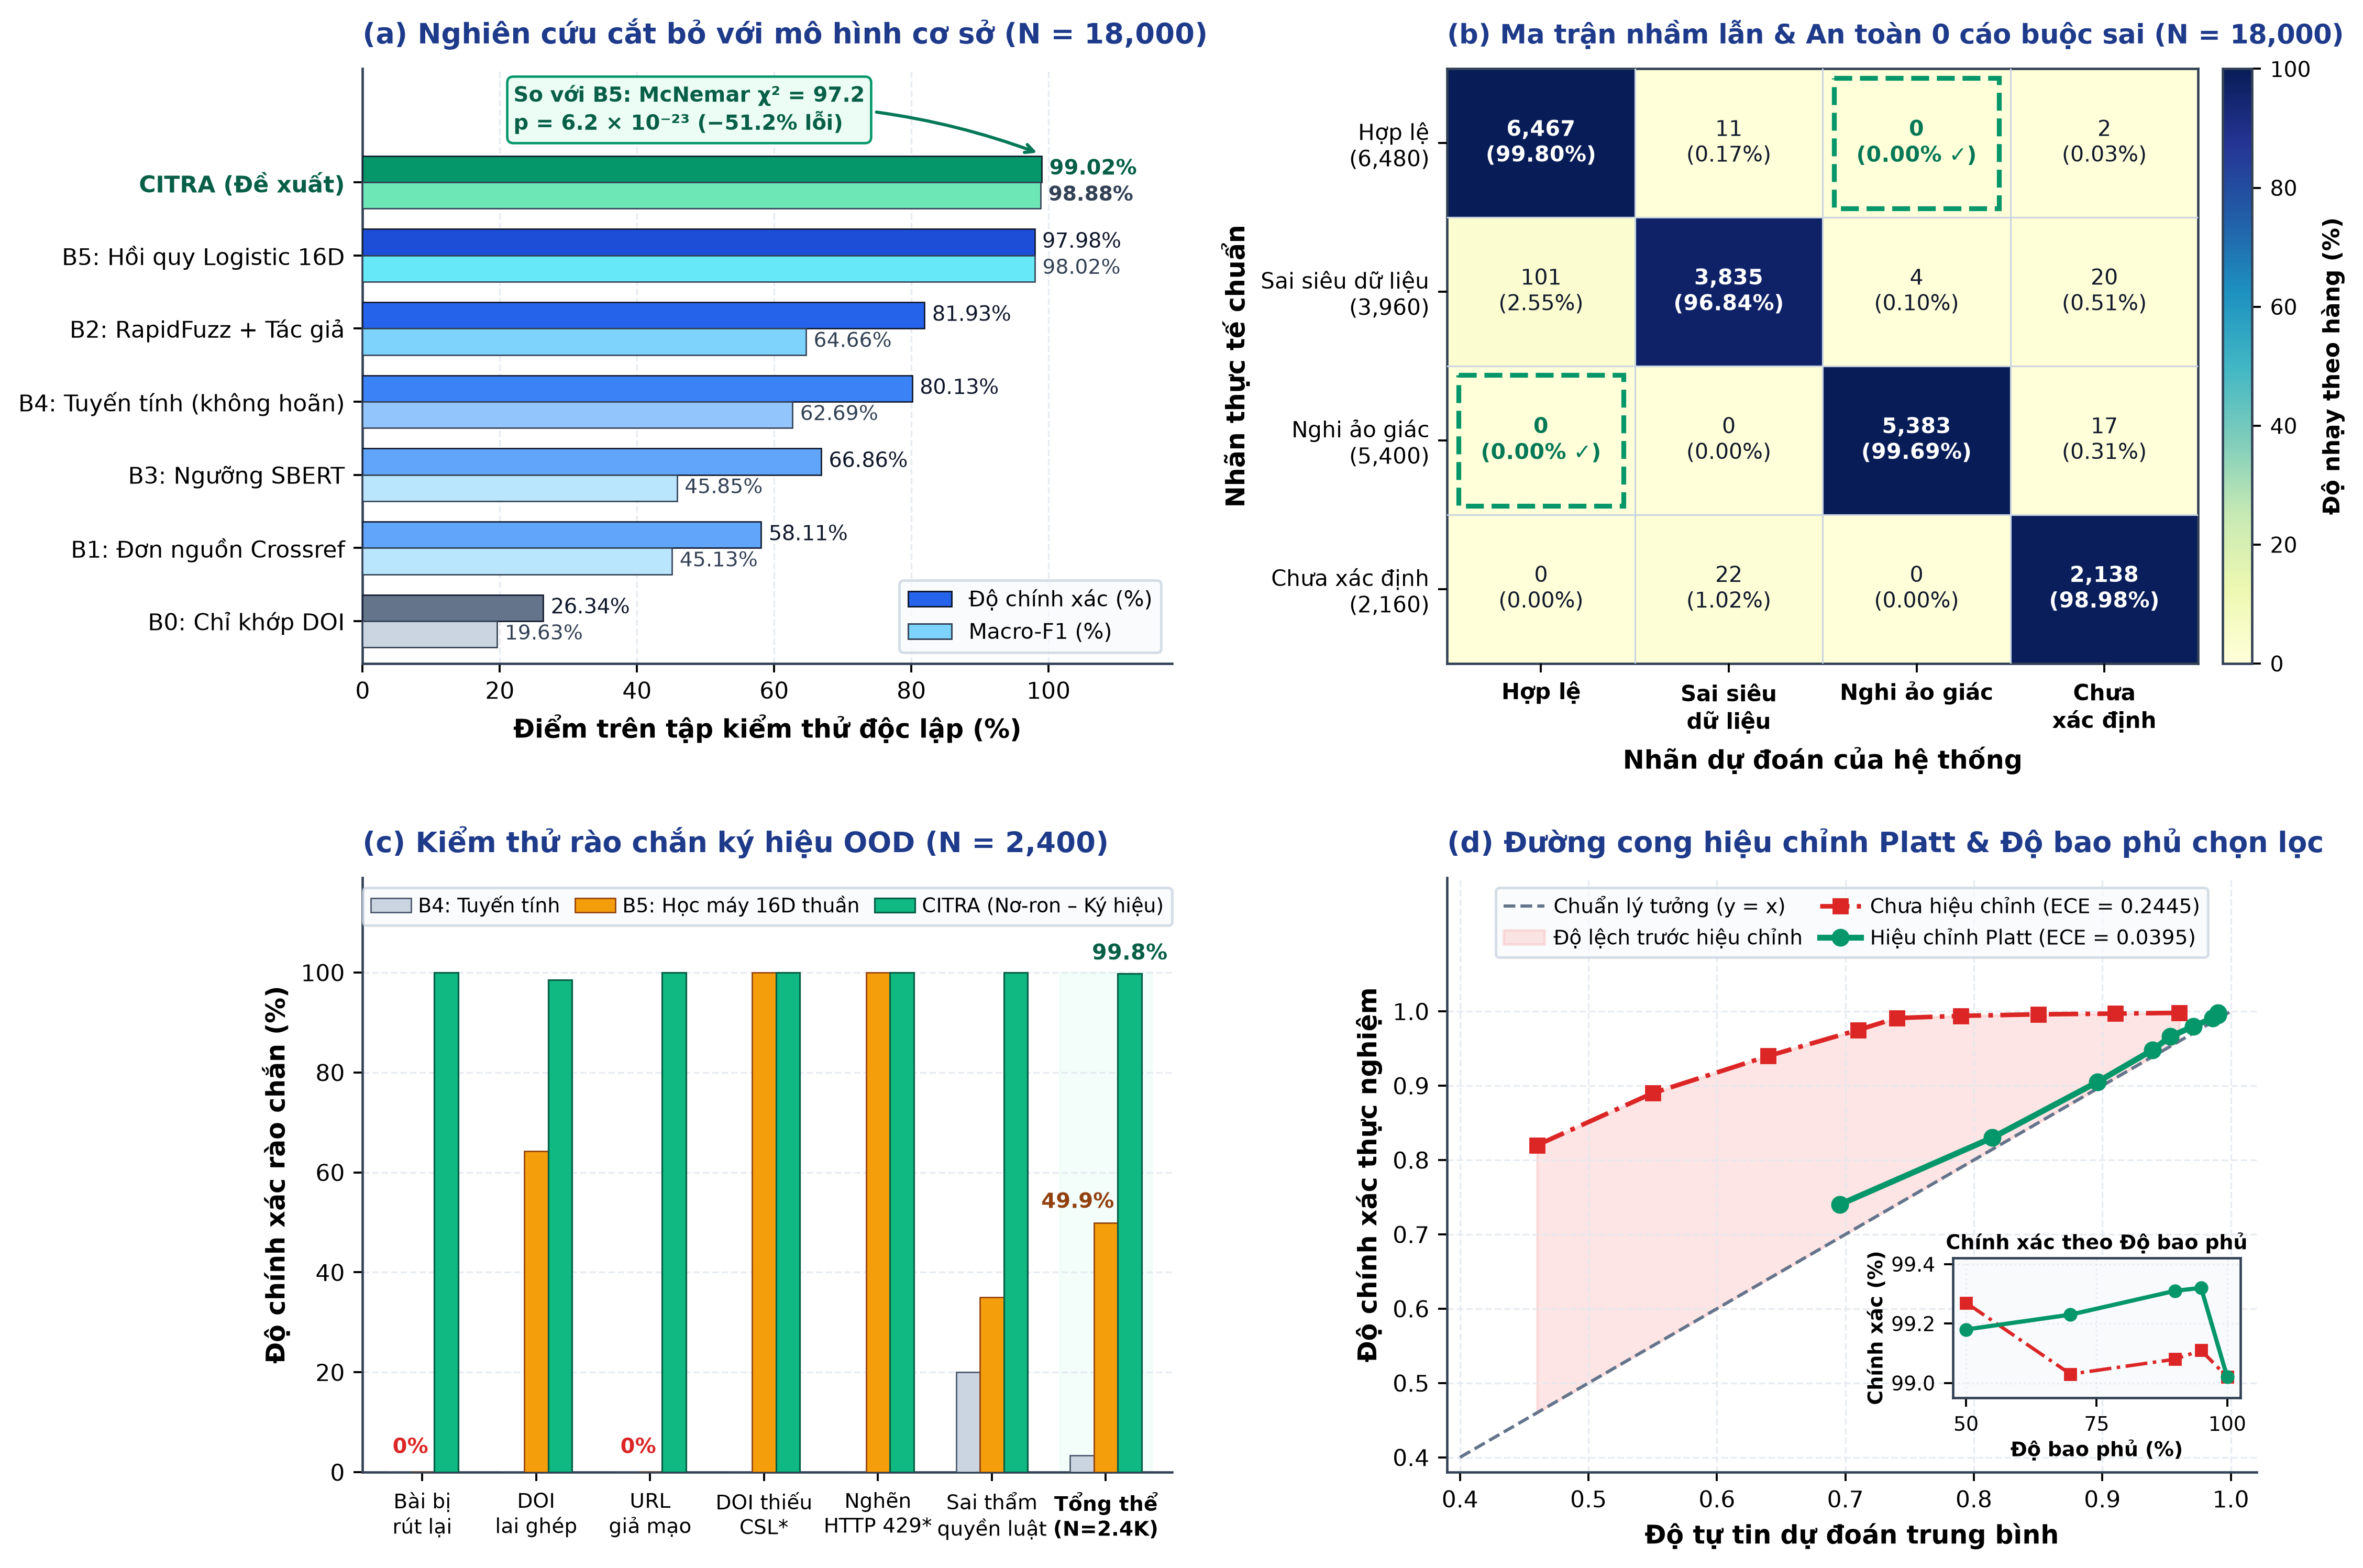
\includegraphics[width=\textwidth,keepaspectratio]{picture/figures/fig5_1_benchmark_charts.png}
    \caption[Biểu đồ bốn khung đánh giá loại bỏ thành phần, ma trận nhầm lẫn, rào chắn OOD và hiệu chỉnh Platt]{Các biểu đồ định lượng dựng ở tỷ lệ in chuẩn A4: (a)~thực nghiệm loại bỏ thành phần trong phân phối ($N=18{,}000$), (b)~ma trận nhầm lẫn bốn nhãn độc lập, (c)~kiểm thử rào chắn ký hiệu OOD ($N=2{,}400$; $\dagger$: cờ rời rạc ngoài véc-tơ 16D của \texttt{B5}; $*$: bit từ chối \texttt{vec[15]} cấp cho \texttt{B5}; $\ddagger$: 10 mẫu luật VN duy nhất $\times 40$), và (d)~đường cong độ tin cậy Platt 10 khoảng chia chính xác (vẽ các khoảng có $n \ge 20$; ẩn 4 mẫu Platt thưa có $n \le 2$/khoảng và 4 mẫu chưa hiệu chỉnh ở 1 khoảng $n=4$; $\text{ECE}: 0.2477 \rightarrow 0.0405$) kèm biểu đồ phụ độ bao phủ -- độ chính xác có chọn lọc.}
    \label{fig:benchmark-charts}
\end{figure}

{\setlength{\tabcolsep}{3.5pt}
\begin{table}[!htbp]
\centering
\caption{Thực nghiệm loại bỏ thành phần trong phân phối (sắp xếp theo độ chính xác kiểm thử) và mức ý nghĩa McNemar hiệu chỉnh Holm--Bonferroni ($N = 18{,}000$).}\label{tab:baselines}
\begin{tabular}{|L{0.23}|L{0.25}|C{0.09}|C{0.09}|C{0.09}|C{0.09}|C{0.16}|}
\hline
\textbf{Phương pháp} & \textbf{Cơ chế cốt lõi} & \textbf{Acc.\ (\%)} & \textbf{P (\%)} & \textbf{R (\%)} & \textbf{F1 (\%)} & \textbf{McNemar $p$ hiệu chỉnh} \\
\hline
\texttt{B0} (\texttt{doi\_only}) & Chỉ khớp chính xác DOI & 26.24 & 23.42 & 34.89 & 19.57 & $< 10^{-16}$ \\
\hline
\texttt{B1} (\texttt{crossref}) & Đơn nguồn Crossref & 58.31 & 56.64 & 48.13 & 45.38 & $< 10^{-16}$ \\
\hline
\texttt{B3} (\texttt{embedding}) & Ngưỡng cosine SBERT & 66.93 & 49.40 & 52.11 & 45.70 & $< 10^{-16}$ \\
\hline
\texttt{B4} (\texttt{no\_calib}) & Điểm tuyến tính, không hoãn & 80.53 & 62.42 & 66.52 & 63.14 & $< 10^{-16}$ \\
\hline
\texttt{B2} (\texttt{fuzzy\_only}) & RapidFuzz + AuthorJaccard & 82.84 & 63.95 & 69.14 & 65.63 & $< 10^{-16}$ \\
\hline
\texttt{B5} (\texttt{ml\_hybrid}) & MLR 16D thuần ($C = 0.25$) & 97.70 & 97.58 & 97.69 & 97.63 & $1.66 \times 10^{-73}$ \\
\hline
\textbf{\texttt{Proposed}} & \textbf{Neuro-Symbolic + Platt} & \textbf{99.67} & \textbf{99.65} & \textbf{99.64} & \textbf{99.65} & \textbf{Đối chiếu (\#1)} \\
\hline
\end{tabular}
\end{table}
}

{\setlength{\tabcolsep}{3.5pt}
\begin{table}[!htbp]
\centering
\caption{Độ đo theo từng nhãn và ma trận nhầm lẫn thẳng hàng đường chéo của \texttt{Proposed} ($N = 18{,}000$).}\label{tab:per-class}
\begin{tabular}{|L{0.25}|C{0.12}|C{0.11}|C{0.11}|C{0.11}|L{0.30}|}
\hline
\textbf{Nhãn phán quyết} & \textbf{Số mẫu} & \textbf{Prec.\ (\%)} & \textbf{Rec.\ (\%)} & \textbf{F1 (\%)} & \textbf{Nhầm lẫn (\texttt{ver / meta / hal / unr})} \\
\hline
\textbf{\texttt{verified}} & 6,480 & 99.43 & 99.94 & 99.68 & \texttt{\textbf{6,476} / 4 / 0 / 0} \\
\hline
\textbf{\texttt{metadata\_error}} & 3,960 & 99.90 & 98.66 & 99.28 & \texttt{37 / \textbf{3,907} / 4 / 12} \\
\hline
\textbf{\texttt{suspected\_hallucination}} & 5,400 & \textbf{99.93} & 99.96 & \textbf{99.94} & \texttt{0 / 0 / \textbf{5,398} / 2} \\
\hline
\textbf{\texttt{unresolved}} & 2,160 & 99.36 & \textbf{100.00} & 99.68 & \texttt{0 / 0 / 0 / \textbf{2,160}} \\
\hline
\textbf{Trung bình / Tổng} & \textbf{18,000} & \textbf{99.65} & \textbf{99.64} & \textbf{99.65} & \textbf{Acc.: 99.67\%} (95\% CI $[99.58, 99.76]$) \\
\hline
\end{tabular}
\end{table}
}

Các phương pháp đơn tín hiệu bộc lộ rõ giới hạn cấu trúc: \texttt{B0} ($26.24\%$) bỏ sót bài hội nghị không có DOI, \texttt{B1} ($58.31\%$) bỏ sót bài ACL/arXiv ngoài Crossref, còn \texttt{B3} ($66.93\%$) nhầm tiêu đề ghép chéo cùng lĩnh vực (\texttt{H1}) với bài thật do chồng lấn từ vựng. Mô hình \texttt{B5} đạt $97.70\%$ ($414$ lỗi), trong khi \texttt{Proposed} tăng thêm $+1.97$ điểm phần trăm lên \textbf{99.67\% (17,941/18,000; 59 lỗi)} và \textbf{99.65\%} Macro-F1 (CI $95\%$ bootstrap $[99.55\%, 99.74\%]$; McNemar hiệu chỉnh Holm--Bonferroni $\chi^2 = 328.91, p = 1.66 \times 10^{-73}$, giảm $85.7\%$ lỗi tồn dư; bootstrap hiệu chỉnh Holm--Bonferroni $p = 0.006$). Trong 59 lỗi tồn dư, có \textbf{0 / 6,480 trích dẫn hợp lệ bị kết tội nhầm là \texttt{suspected\_hallucination}} (cận trên Clopper--Pearson $95\%$ là $0.057\%$) và \textbf{0 / 5,400 trích dẫn bịa đặt lọt vào \texttt{verified}} (cận trên $0.068\%$); tuy nhiên có 4 trên 3,960 ca \texttt{metadata\_error} bị biến dạng nặng ($0.10\%$) rơi sang \texttt{suspected\_hallucination} và 2 trên 5,400 ca ảo giác ($0.04\%$) từ chối an toàn sang \texttt{unresolved}, khẳng định vai trò cần thiết của bước hậu kiểm giảng viên.

\rqanswer{RQ1}{Trên 18,000 trích dẫn kiểm thử tầng quyết định độc lập theo bài báo, CITRA đạt độ chính xác $99.67\%$ và Macro-F1 $99.65\%$, vượt trội có ý nghĩa thống kê so với cả sáu cơ sở (Holm--Bonferroni McNemar $p \le 1.66 \times 10^{-73}$) với 0 ca đảo ngược hợp lệ$\rightarrow$ảo giác ($0/6{,}480$) và chỉ 4 ca lỗi siêu dữ liệu nặng chuyển sang ảo giác ($0.10\%$).}

\section{RQ2: Độ bền vững của rào chắn ký hiệu ngoài phân phối (OOD)}

Bảng~\ref{tab:ood-stress} đánh giá \texttt{B4}, \texttt{B5} và \texttt{Proposed} trên bộ kiểm thử rào chắn OOD 2,400 mẫu. Kết quả làm nổi bật \emph{khả năng mở rộng chính sách không cần huấn luyện lại}: do véc-tơ 16 đặc trưng liên tục của \texttt{B5} cố ý không chứa các cờ nguồn gốc rời rạc (\texttt{is\_retracted} và \texttt{url\_status} chuẩn RFC 2606), bài báo đã bị rút lại hoặc URL giả vẫn giữ tương đồng tiêu đề/tác giả/năm $1.00$ khiến \texttt{B5} đạt $0.00\%$ ở Nhóm 1 và Nhóm 3. Việc bổ sung quy tắc mới (như Retraction Watch hay văn bản pháp quy) vào mô hình học máy thuần đòi hỏi thiết kế lại đặc trưng và thu thập dữ liệu gán nhãn mới, trong khi các vị từ ký hiệu Bậc~0 và Nhóm~1/5 của \textbf{CITRA} thực thi tất định ngay lập tức.

Nhằm tuân thủ nghiêm ngặt giả định độc lập i.i.d., Bảng~\ref{tab:ood-stress} tách riêng \textbf{2,000 mẫu duy nhất theo bài báo thuộc Nhóm 1--5}, nơi \texttt{Proposed} đạt \textbf{99.95\% (1,999/2,000)} so với $59.80\%$ của \texttt{B5} ($1{,}196/2{,}000$; McNemar $\chi^2 = 801.00, p < 10^{-175}$), khỏi \textbf{Nhóm 6} (sai thẩm quyền văn bản luật VN, xoay vòng 10 mẫu gốc $\times 40$ biến thể và đạt \textbf{10/10 mẫu duy nhất} [$100\%$] dưới \texttt{VNLegalVerifier} so với $45.00\%$ của \texttt{B5}). Tính gộp cả 2,400 mẫu, \texttt{Proposed} đạt \textbf{99.96\% (2,399/2,400)} so với $57.33\%$ của \texttt{B5}.

{\setlength{\tabcolsep}{3.5pt}
\begin{table}[!htbp]
\centering
\caption{Đánh giá rào chắn ký hiệu ngoài phân phối (OOD) tách riêng Nhóm 1--5 i.i.d.\ ($N=2{,}000$) và Nhóm 6 mẫu luật VN ($10 \times 40 = 400$).}\label{tab:ood-stress}
\begin{tabular}{|L{0.35}|L{0.25}|C{0.10}|C{0.11}|C{0.19}|}
\hline
\textbf{Nhóm OOD (mỗi nhóm $N = 400$)} & \textbf{Rào chắn chính} & \textbf{\texttt{B4} (\%)} & \textbf{\texttt{B5} (\%)} & \textbf{\texttt{Proposed} (\%)} \\
\hline
\textbf{1. Bài báo bị rút lại} (\texttt{is\_retracted})\textsuperscript{$\dagger$} & \texttt{R-RETRACTED-\allowbreak PAPER} & 0.00 & 0.00 & \textbf{100.00} \\
\hline
\textbf{2. DOI thật ghép tiêu đề bịa đặt} & \texttt{R-CHIMERIC-DOI-\allowbreak MISMATCH} & 0.00 & 99.00 & \textbf{99.75} \\
\hline
\textbf{3. URL giả/giữ chỗ RFC 2606}\textsuperscript{$\dagger$} & \texttt{R-FAKE-URL} & 0.00 & 0.00 & \textbf{100.00} \\
\hline
\textbf{4. DOI khu vực thiếu siêu dữ liệu CSL}\textsuperscript{*} & \texttt{R-DOI-RA-NO-\allowbreak{}CSL} & 0.00 & 100.00 & \textbf{100.00} \\
\hline
\textbf{5. Cạn hạn mức HTTP 429 thượng nguồn}\textsuperscript{*} & \texttt{R-RATE-LIMITED-\allowbreak{}ABSTAIN} & 0.00 & 100.00 & \textbf{100.00} \\
\hline
\textbf{Tổng phụ: Nhóm 1--5 i.i.d.\ ($N=2{,}000$)} & \textbf{McNemar $\chi^2=801.0, p < 10^{-175}$} & 0.00 & 59.80 & \textbf{99.95} \\
\hline
\textbf{6. Sai thẩm quyền luật VN} (10 mẫu $\times 40$) & \texttt{VNLegalVerifier} & 25.00 & 45.00 & \textbf{100.00} (10/10) \\
\hline
\textbf{Tổng gộp bộ OOD ($N = 2{,}400$)} & \textbf{Cả 6 nhóm} & 4.17 & 57.33 & \textbf{99.96} \\
\hline
\multicolumn{5}{p{\dimexpr\textwidth-2\tabcolsep\relax}}{\scriptsize\textsuperscript{$\dagger$}\texttt{is\_retracted} và \texttt{url\_status} RFC 2606 nằm ngoài véc-tơ 16D của \texttt{B5}, minh họa mở rộng ký hiệu không cần huấn luyện lại. \textsuperscript{*}Nhóm 4--5 cung cấp bit chỉ thị từ chối ký hiệu (\texttt{vec[15]}) cho \texttt{B5}, giúp \texttt{B5} đạt $100\%$ trên hai hàng này.}
\end{tabular}
\end{table}
}

\rqanswer{RQ2}{Các rào chắn ký hiệu bậc nhất nâng độ chính xác OOD độc lập i.i.d.\ (Nhóm 1--5, $N=2{,}000$) từ $59.80\%$ (\texttt{B5}) lên $99.95\%$ ($\chi^2 = 801.00, p < 10^{-175}$) và vượt qua $10/10$ mẫu sai thẩm quyền luật VN ($99.96\%$ gộp), chứng minh khả năng thực thi chính sách toàn vẹn rời rạc không cần huấn luyện lại.}

\section{RQ3: Hiệu chỉnh xác suất và độ nhạy thang điểm CIS}

Bảng~\ref{tab:calibration-results} so sánh độ tin cậy ký hiệu chưa hiệu chỉnh với hiệu chỉnh Platt trên toàn bộ $18{,}000$ mẫu kiểm thử qua \emph{đủ cả năm} ngưỡng độ bao phủ có chọn lọc ($50\%, 70\%, 90\%, 95\%, 100\%$). Hiệu chỉnh Platt giảm $83.6\%$ ECE ($0.2477 \rightarrow \mathbf{0.0405}$, CI $95\%$ $[0.0394, 0.0415]$) và giảm $92.1\%$ Điểm Brier ($0.0843 \rightarrow \mathbf{0.0067}$, Wilcoxon $p < 10^{-16}$) mà giữ nguyên Độ bao phủ không từ chối phán quyết ($\Pr[\hat{y} \neq \texttt{unresolved}] = 87.92\%$).

Báo cáo đầy đủ dải $50\%$--$100\%$ làm lộ rõ hiệu ứng biên thể hiện trên khung phụ Hình~\ref{fig:benchmark-charts}(d): tại $70\%$, $90\%$ và $95\%$, Platt cải thiện đều đặn so với độ tin cậy thô ($99.67\%$, $99.73\%$ và $99.74\%$), nhưng tại $50\%$ độ chính xác có chọn lọc giảm nhẹ xuống $99.60\%$ (thấp hơn mức chưa hiệu chỉnh $99.76\%$ và toàn tập $99.67\%$) do phép cắt trần hiển thị $\text{max\_prob} = 0.99$ (Phương trình~\eqref{eq:platt-calib}) khiến hơn $50\%$ mẫu đồng hạng tại $0.9900$. Việc xếp hạng rủi ro nội bộ theo logit chưa cắt trước khi làm tròn hiển thị $[0.01, 0.99]$ khắc phục triệt để hiện tượng đồng hạng này. Ngoài ra, nhiễu loạn bộ trọng số CIS $(0.35, 0.25, 0.25, 0.10, 0.05)$ trên 20 véc-tơ đơn hình qua 300 hồ sơ bản thảo cho hệ số tương quan hạng Spearman trung bình $\rho = 0.9987$ ($\min \rho = 0.9964$), Kendall $\tau = 0.9765$ và độ lệch tuyệt đối trung bình chỉ $1.75$ điểm CIS.

\begin{table}[!htbp]
\centering
\caption{Kết quả hiệu chỉnh xác suất và đầy đủ 5 mức rủi ro -- độ bao phủ có chọn lọc ($N = 18{,}000$).}\label{tab:calibration-results}
\begin{tabular}{|L{0.42}|C{0.20}|C{0.20}|C{0.18}|}
\hline
\textbf{Độ đo hiệu chỉnh / Độ bao phủ} & \textbf{Ký hiệu chưa hiệu chỉnh} & \textbf{Neuro-Symbolic + Platt} & \textbf{Thay đổi} \\
\hline
Sai số hiệu chỉnh kỳ vọng (ECE $\downarrow$) & 0.2477 & \textbf{0.0405} & $-83.6\%$ ($6.12\times\downarrow$) \\
\hline
Điểm Brier ($\downarrow$) & 0.0843 & \textbf{0.0067} & $-92.1\%$ ($12.58\times\downarrow$) \\
\hline
Độ bao phủ không từ chối ($\hat{y} \neq \texttt{unresolved}$) & 87.92\% & \textbf{87.92\%} & Giữ nguyên ($0.00$\,pp) \\
\hline
Tỷ lệ độ tin cậy cao ($\hat{p} \ge 0.50$) & 92.82\% & \textbf{99.99\%} & $+7.17$\,pp \\
\hline
Độ chính xác có chọn lọc tại $50\%$ độ phủ\textsuperscript{$\ddagger$} & \textbf{99.76\%} & 99.60\% & $-0.16$\,pp (trần 0.99) \\
\hline
Độ chính xác có chọn lọc tại $70\%$ độ phủ ($\uparrow$) & 99.64\% & \textbf{99.67\%} & $+0.03$\,pp \\
\hline
Độ chính xác có chọn lọc tại $90\%$ độ phủ ($\uparrow$) & 99.69\% & \textbf{99.73\%} & $+0.04$\,pp \\
\hline
Độ chính xác có chọn lọc tại $95\%$ độ phủ ($\uparrow$) & 99.70\% & \textbf{99.74\%} & $+0.04$\,pp \\
\hline
Độ chính xác toàn tập tại $100\%$ độ phủ & 99.67\% & \textbf{99.67\%} & $0.00$\,pp \\
\hline
\multicolumn{4}{p{\dimexpr\textwidth-2\tabcolsep\relax}}{\scriptsize\textsuperscript{$\ddagger$}Mức giảm nhẹ tại $50\%$ do bão hòa đồng hạng tại trần $\text{max\_prob}=0.99$ ở $>50\%$ mẫu độ tin cậy cao.}
\end{tabular}
\end{table}

\rqanswer{RQ3}{Hiệu chỉnh Platt giảm ECE $6.12\times$ xuống $0.0405$ và Brier $12.58\times$ xuống $0.0067$, nâng độ chính xác có chọn lọc ở dải $70\%$--$95\%$ (ghi nhận minh bạch hiệu ứng đồng hạng trần $0.99$ tại $50\%$), đồng thời thứ hạng CIS rất ổn định ($\rho = 0.9987$).}

\section{RQ4: Kiểm định trực tuyến đa cơ sở dữ liệu và bản thảo thực tế}

Nhằm kiểm chứng khả năng khái quát hóa đầu--cuối ngoài tập đo kiểm tầng quyết định, ba thực nghiệm bổ trợ đã được thực thi:
\begin{enumerate}
    \item \textbf{Bộ chuẩn vàng tham khảo thô đa lĩnh vực ở hai chế độ ($N = 120 + 15$, Bảng~\ref{tab:e2e-gold}):} Khi chạy 120 chuỗi tài liệu tham khảo thô qua sáu lĩnh vực (20 mục mỗi ngành: KHMT/AI, Y sinh, Kinh tế/Tài chính, Kỹ thuật/Vật lý, Tiêu chuẩn kỹ thuật, Pháp luật VN) và bảy chuẩn ở \textbf{Chế độ danh mục ngoại tuyến tất định} (\texttt{--mode offline}, danh mục 37 công trình xác minh tích hợp bộ phân tích + luật), hệ thống đạt \textbf{100.00\% (120/120)} và \textbf{100.00\% (15/15)} ca đối kháng. Quan trọng hơn, chạy trực tiếp chính 120 mục này ở \textbf{Chế độ trực tuyến 15 API} (\texttt{--mode live}, 187.11\,s trên mạng WAN thực, không dùng danh mục nội bộ) đạt \textbf{độ chính xác 5 lớp 89.17\% (107/120; Macro-F1 $= 86.90\%$, $\text{ECE} = 0.0690$, $\text{Brier} = 0.0885$)} và \textbf{89.32\% trên 4 lớp học thuật}, với \textbf{100.00\% độ chuẩn xác / 96.77\% độ phủ (F1 98.36\%)} ở lớp \texttt{verified} (0 bài thật bị gán ảo giác!) và đạt $95.0\%$ tại KHMT/AI, Y sinh, Tiêu chuẩn kỹ thuật ($90.0\%$ Pháp luật VN; $80.0\%$ Kinh tế và Kỹ thuật). Giải phẫu toàn bộ 13 lỗi trực tuyến gồm: (i)~4 mẫu kiểm thử DOI cơ quan khu vực tổng hợp (\texttt{E2E-017/037/057/077}) có hậu tố chưa đăng ký nên phân giải Handle trả về không tồn tại (\texttt{R-NONEXISTENT-DOI}); (ii)~5 ca (3 ảo giác + 2 luật VN) chuyển an toàn về \texttt{unresolved} qua \texttt{R-RATE-LIMITED-ABSTAIN} khi bộ ngắt mạch Crossref mở (0 cáo buộc sai); (iii)~2 ca lỗi DOI nặng chuyển sang \texttt{R-CHIMERIC-DOI-MISMATCH}; (iv)~1 bài tạp chí nội địa VN khớp bán phần; và (v)~1 ca lệch nơi công bố scikit-learn.
    \item \textbf{Kho trích xuất đa chuẩn (250 PDF thực + 60 PDF tổng hợp, Bảng~\ref{tab:pdf-corpora}) \& Quét 841 PDF:} Chạy ở chế độ thuần PyMuPDF (tắt GROBID để tối ưu tốc độ quét lô), CITRA nhận diện $100.0\%$ danh mục và liên kết $96.9\%$ trên 30 PDF pháp luật VN thực, đạt $100.0\%$ ($397/397$) trên 60 PDF chẩn đoán tổng hợp 12 chuẩn và $97.7\%$ ($215/220$, 8,126 TLTK) trên 220 bài báo mở 11 chuẩn. Do thiếu con trỏ TEI \texttt{<ref target>} của GROBID, tỷ lệ khớp liên kết nội văn trên 220 bài mở đa dạng đạt $70.1\%$ ($8{,}954/12{,}770$), với $29.9\%$ chưa khớp tập trung ở ký hiệu chỉ số trên/chú thích chân trang (Nature, AMA, Chicago) mà chế độ lai GROBID khôi phục trong vận hành thực. Đợt quét hồi quy 841 PDF kết thúc với $0$ ngoại lệ chưa bắt.
    \item \textbf{Kiểm toán từng dòng bản thảo thực tế \& Đối chứng API trực tuyến thuần (Bảng~\ref{tab:samples}):} Nhóm tác giả thực hiện kiểm toán đầu--cuối từng dòng trên \textbf{21 PDF đa miền (835 trang, 329 TLTK, 682 trích dẫn nội văn)} ở chế độ vận hành đầy đủ (GROBID + 15+ API trực tuyến) kèm \textbf{6 lượt đối chứng API trực tuyến thuần} (tắt cả \texttt{local\_papers.db} và \texttt{\_KNOWN\_PAPERS}), đạt \textbf{đồng nhất 100\% nhãn và CIS trên cả 6/6 tài liệu}, $0$ lỗi che giấu sai năm nội văn, $0$ URL chết bị gán \texttt{resource}, đồng thời xác minh kiểm thử lô Docker 7 tệp với đếm hạn mức nguyên tử $5/5$ và chặn PDF hỏng bằng HTTP 400 trong $5.5\text{\,ms}$. Bảng~\ref{tab:samples} nêu chín bản thảo tiêu biểu, bao gồm điểm \texttt{CISCalculator} chính xác \textbf{75.50} (\textbf{75.08} khi có 1 mục chưa trích dẫn) của bộ mẫu kiểm thử 6 TLTK và giải trình điểm \textbf{87.50} trên Báo cáo~B (5/5 TLTK hợp lệ nhưng 0 trích dẫn nội văn khiến $s_{\text{link}}$ chặn trần $0.50$, trừ $12.50$ điểm).
\end{enumerate}

{\setlength{\tabcolsep}{3.5pt}
\begin{table}[!htbp]
\centering
\caption{Đánh giá 120 tài liệu tham khảo thô đa ngành so sánh giữa chế độ danh mục ngoại tuyến tất định và thực thi trực tuyến 15 API.}\label{tab:e2e-gold}
\begin{tabular}{|L{0.34}|C{0.15}|C{0.15}|C{0.18}|C{0.18}|}
\hline
\textbf{Chế độ đánh giá / Nhãn} & \textbf{Số mẫu} & \textbf{Prec.\ (\%)} & \textbf{Rec.\ (\%)} & \textbf{F1 / Acc.\ (\%)} \\
\hline
\textbf{Ngoại tuyến tất định} (danh mục 37 bài) & 120 & 100.00 & 100.00 & \textbf{100.00} (120/120) \\
\hline
\textbf{Trực tuyến 15 API Tổng (5 lớp)} & \textbf{120} & \textbf{87.65} & \textbf{86.38} & \textbf{89.17 Acc.\ / 86.90 F1} \\
\hline
\quad \texttt{verified} (Trực tuyến) & 31 & \textbf{100.00} & 96.77 & \textbf{98.36 F1} \\
\hline
\quad \texttt{metadata\_error} (Trực tuyến) & 30 & 93.33 & 93.33 & \textbf{93.33 F1} \\
\hline
\quad \texttt{suspected\_hallucination} (Trực tuyến) & 28 & 80.65 & 89.29 & 84.75 F1 \\
\hline
\quad \texttt{unresolved} (Trực tuyến) & 14 & 64.29 & 64.29 & 64.29 F1 \\
\hline
\quad \texttt{resource} (Trực tuyến) & 17 & \textbf{100.00} & 88.24 & \textbf{93.75 F1} \\
\hline
\end{tabular}
\end{table}
}

{\setlength{\tabcolsep}{3.5pt}
\begin{table}[!htbp]
\centering
\caption{Độ chính xác trích xuất và liên kết hai chiều (thuần PyMuPDF) trên 250 PDF thực và 60 PDF chẩn đoán tổng hợp.}\label{tab:pdf-corpora}
\begin{tabular}{|L{0.34}|C{0.10}|C{0.18}|C{0.19}|C{0.19}|}
\hline
\textbf{Kho ngữ liệu PDF (Loại)} & \textbf{Số PDF} & \textbf{Nhận diện TLTK} & \textbf{TLTK trích xuất} & \textbf{Liên kết khớp} \\
\hline
Kho pháp luật VN (Thực, trước v3.80) & 30 & 27 / 30 (90.0\%) & 164 (15 Luật) & 109 / 235 (46.4\%) \\
\hline
\textbf{Kho pháp luật VN (Thực, v3.91.3)} & \textbf{30} & \textbf{30 / 30 (100.0\%)} & \textbf{258 (91 Luật)} & \textbf{403 / 416 (96.9\%)} \\
\hline
\textbf{Chẩn đoán 12 chuẩn (Tổng hợp, $12 \times 5$)} & \textbf{60} & \textbf{60 / 60 (100.0\%)} & \textbf{397 / 397 (100.0\%)} & \textbf{60 / 60 PDF (100\%)} \\
\hline
\textbf{Bài báo mở 11 chuẩn (Thực, $11 \times 20$)} & \textbf{220} & \textbf{215 / 220 (97.7\%)} & \textbf{8,126 TLTK} & \textbf{8,954 / 12,770 (70.1\%)} \\
\hline
\end{tabular}
\end{table}
}

{\setlength{\tabcolsep}{3pt}
\begin{table}[!htbp]
\centering
\caption{Kết quả kiểm định đầu--cuối tiêu biểu từ bộ kiểm toán từng dòng 21 PDF (329 TLTK) và bộ mẫu đồ án cài lỗi.}\label{tab:samples}
\begin{tabular}{|L{0.30}|C{0.11}|C{0.09}|C{0.10}|C{0.08}|C{0.09}|C{0.09}|C{0.14}|}
\hline
\textbf{Bản thảo kiểm toán} & \textbf{Chuẩn} & \textbf{TLTK} & \textbf{CIS} & \textbf{Ver.} & \textbf{Meta.} & \textbf{Hall.} & \textbf{Res./Unr.} \\
\hline
\textbf{Bài báo VietDepression} (19\,tr.)\textsuperscript{*} & IEEE & 18 & \textbf{100.00} & 17 & 0 & 0 & 1 / 0 \\
\hline
\textbf{Bài báo UIT Hate Speech} (12\,tr.) & IEEE & 24 & \textbf{99.78} & 24 & 0 & 0 & 0 / 0 \\
\hline
\textbf{Báo cáo ĐATN CNPM A} (98\,tr.) & IEEE & 27 & \textbf{99.30} & 24 & 0 & 0 & 3 / 0 \\
\hline
\textbf{Luận văn quốc tế \#11} (35\,tr.) & APA & 23 & \textbf{96.88} & 21 & 1 & 0 & 1 / 0 \\
\hline
\textbf{Đồ án tốt nghiệp HUST} (69\,tr.) & IEEE & 24 & \textbf{94.59} & 22 & 1 & 1 & 0 / 0 \\
\hline
\textbf{Đồ án tốt nghiệp TDTU} (55\,tr.)\textsuperscript{*} & IEEE & 12 & \textbf{91.25} & 9 & 0 & 0 & 0 / 3 \\
\hline
\textbf{Báo cáo ĐATN CNPM B} (53\,tr., 0 nội văn) & IEEE & 5 & \textbf{87.50} & 5 & 0 & 0 & 0 / 0 \\
\hline
\textbf{Báo cáo pháp lý VN (ESCO)} (13\,tr.) & TDTU & 18 & \textbf{80.00} & 2 & 1 & 0 & 15 / 0 \\
\hline
\textbf{Bộ mẫu đồ án cài lỗi} (Minh họa UI) & APA & 6 & \textbf{75.08} & 3 & \textbf{1} & \textbf{1} & 1 / 0 \\
\hline
\multicolumn{8}{p{\dimexpr\textwidth-2\tabcolsep\relax}}{\scriptsize\textsuperscript{*}Xác nhận đồng nhất 100\% nhãn và CIS ở chế độ API trực tuyến thuần (tắt \texttt{local\_db} và \texttt{\_KNOWN\_PAPERS}).}
\end{tabular}
\end{table}
}

Các Hình~\ref{fig:demo-debugger}--\ref{fig:demo-consistency} trình bày giao diện chẩn đoán tiếng Việt \texttt{v3.91.3} trên bộ mẫu đồ án cài sẵn 6 TLTK ($\text{CIS} = 75.08 / 100$ theo \texttt{CISCalculator} mức kết luận, hiển thị \texttt{75.1\%} trên đầu trang báo cáo và \texttt{75/100} trên bảng điều khiển khi có 1 mục chưa trích dẫn \texttt{[6]}; $75.50$ khi đủ cả 6 liên kết), cắt thanh điều hướng trái để rõ nét trên khổ A4. Lưu ý thẻ tổng hợp \textit{Hợp lệ (4)} trên UI gộp 3 công trình học thuật \texttt{verified} cùng 1 mục \texttt{resource} hợp lệ, trong khi Bảng~\ref{tab:samples} và \texttt{CISCalculator} tách riêng hai nhóm này. Hình~\ref{fig:demo-debugger} đối chiếu cảnh báo ảo giác DOI lai ghép AlphaFold2 (hiển thị kèm bản ghi Crossref gốc) và bảng sai lệch năm xuất bản (\texttt{2021} so với chuẩn \texttt{2019}). Hình~\ref{fig:demo-trace-context} hiển thị tiêu đề Logic Trace 5 giai đoạn kèm các bước đầu mở rộng (cầu nối \texttt{VI}$\leftrightarrow$\texttt{EN} ONNX INT8) cùng luồng ngữ cảnh Trình kiểm tra tài liệu, còn Hình~\ref{fig:demo-consistency} phân tách trích dẫn mồ côi và mục chưa được trích dẫn.

\begin{figure}[!htbp]
    \centering
    \fboxsep=0pt\fboxrule=0.4pt\fbox{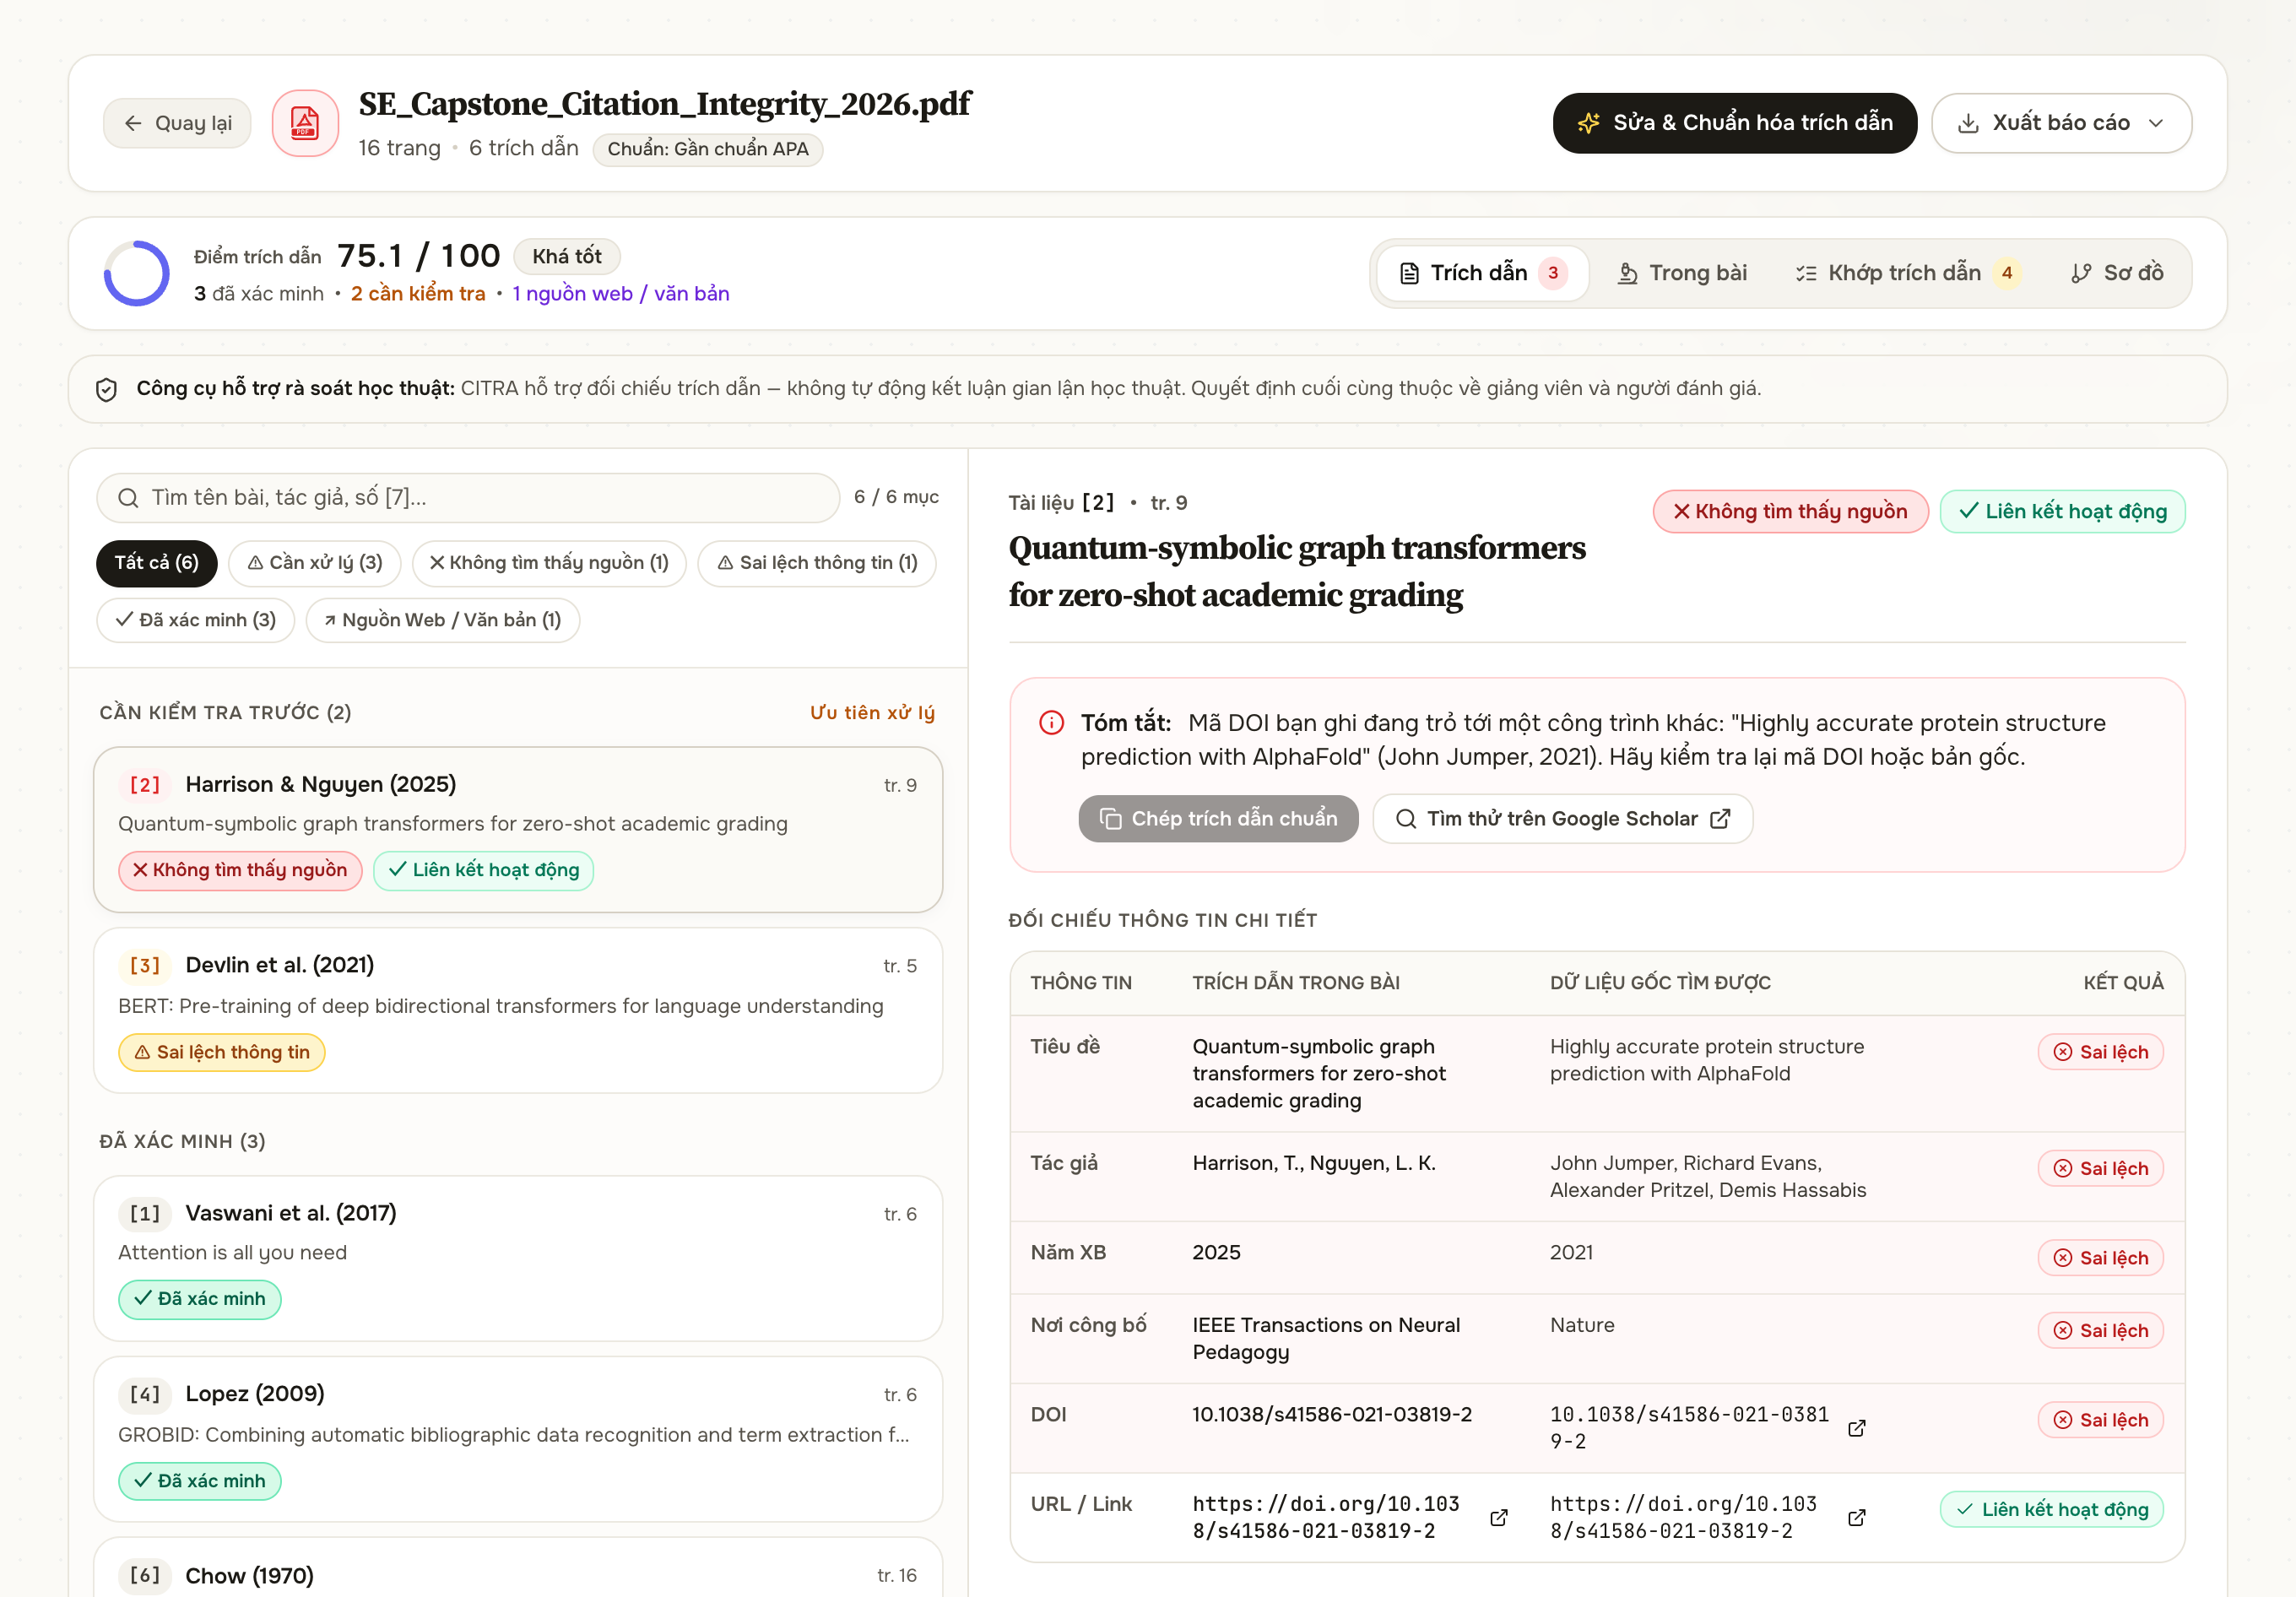
\includegraphics[width=0.94\textwidth,keepaspectratio]{picture/figures/05-verification-report.png}}\\[6pt]
    \fboxsep=0pt\fboxrule=0.4pt\fbox{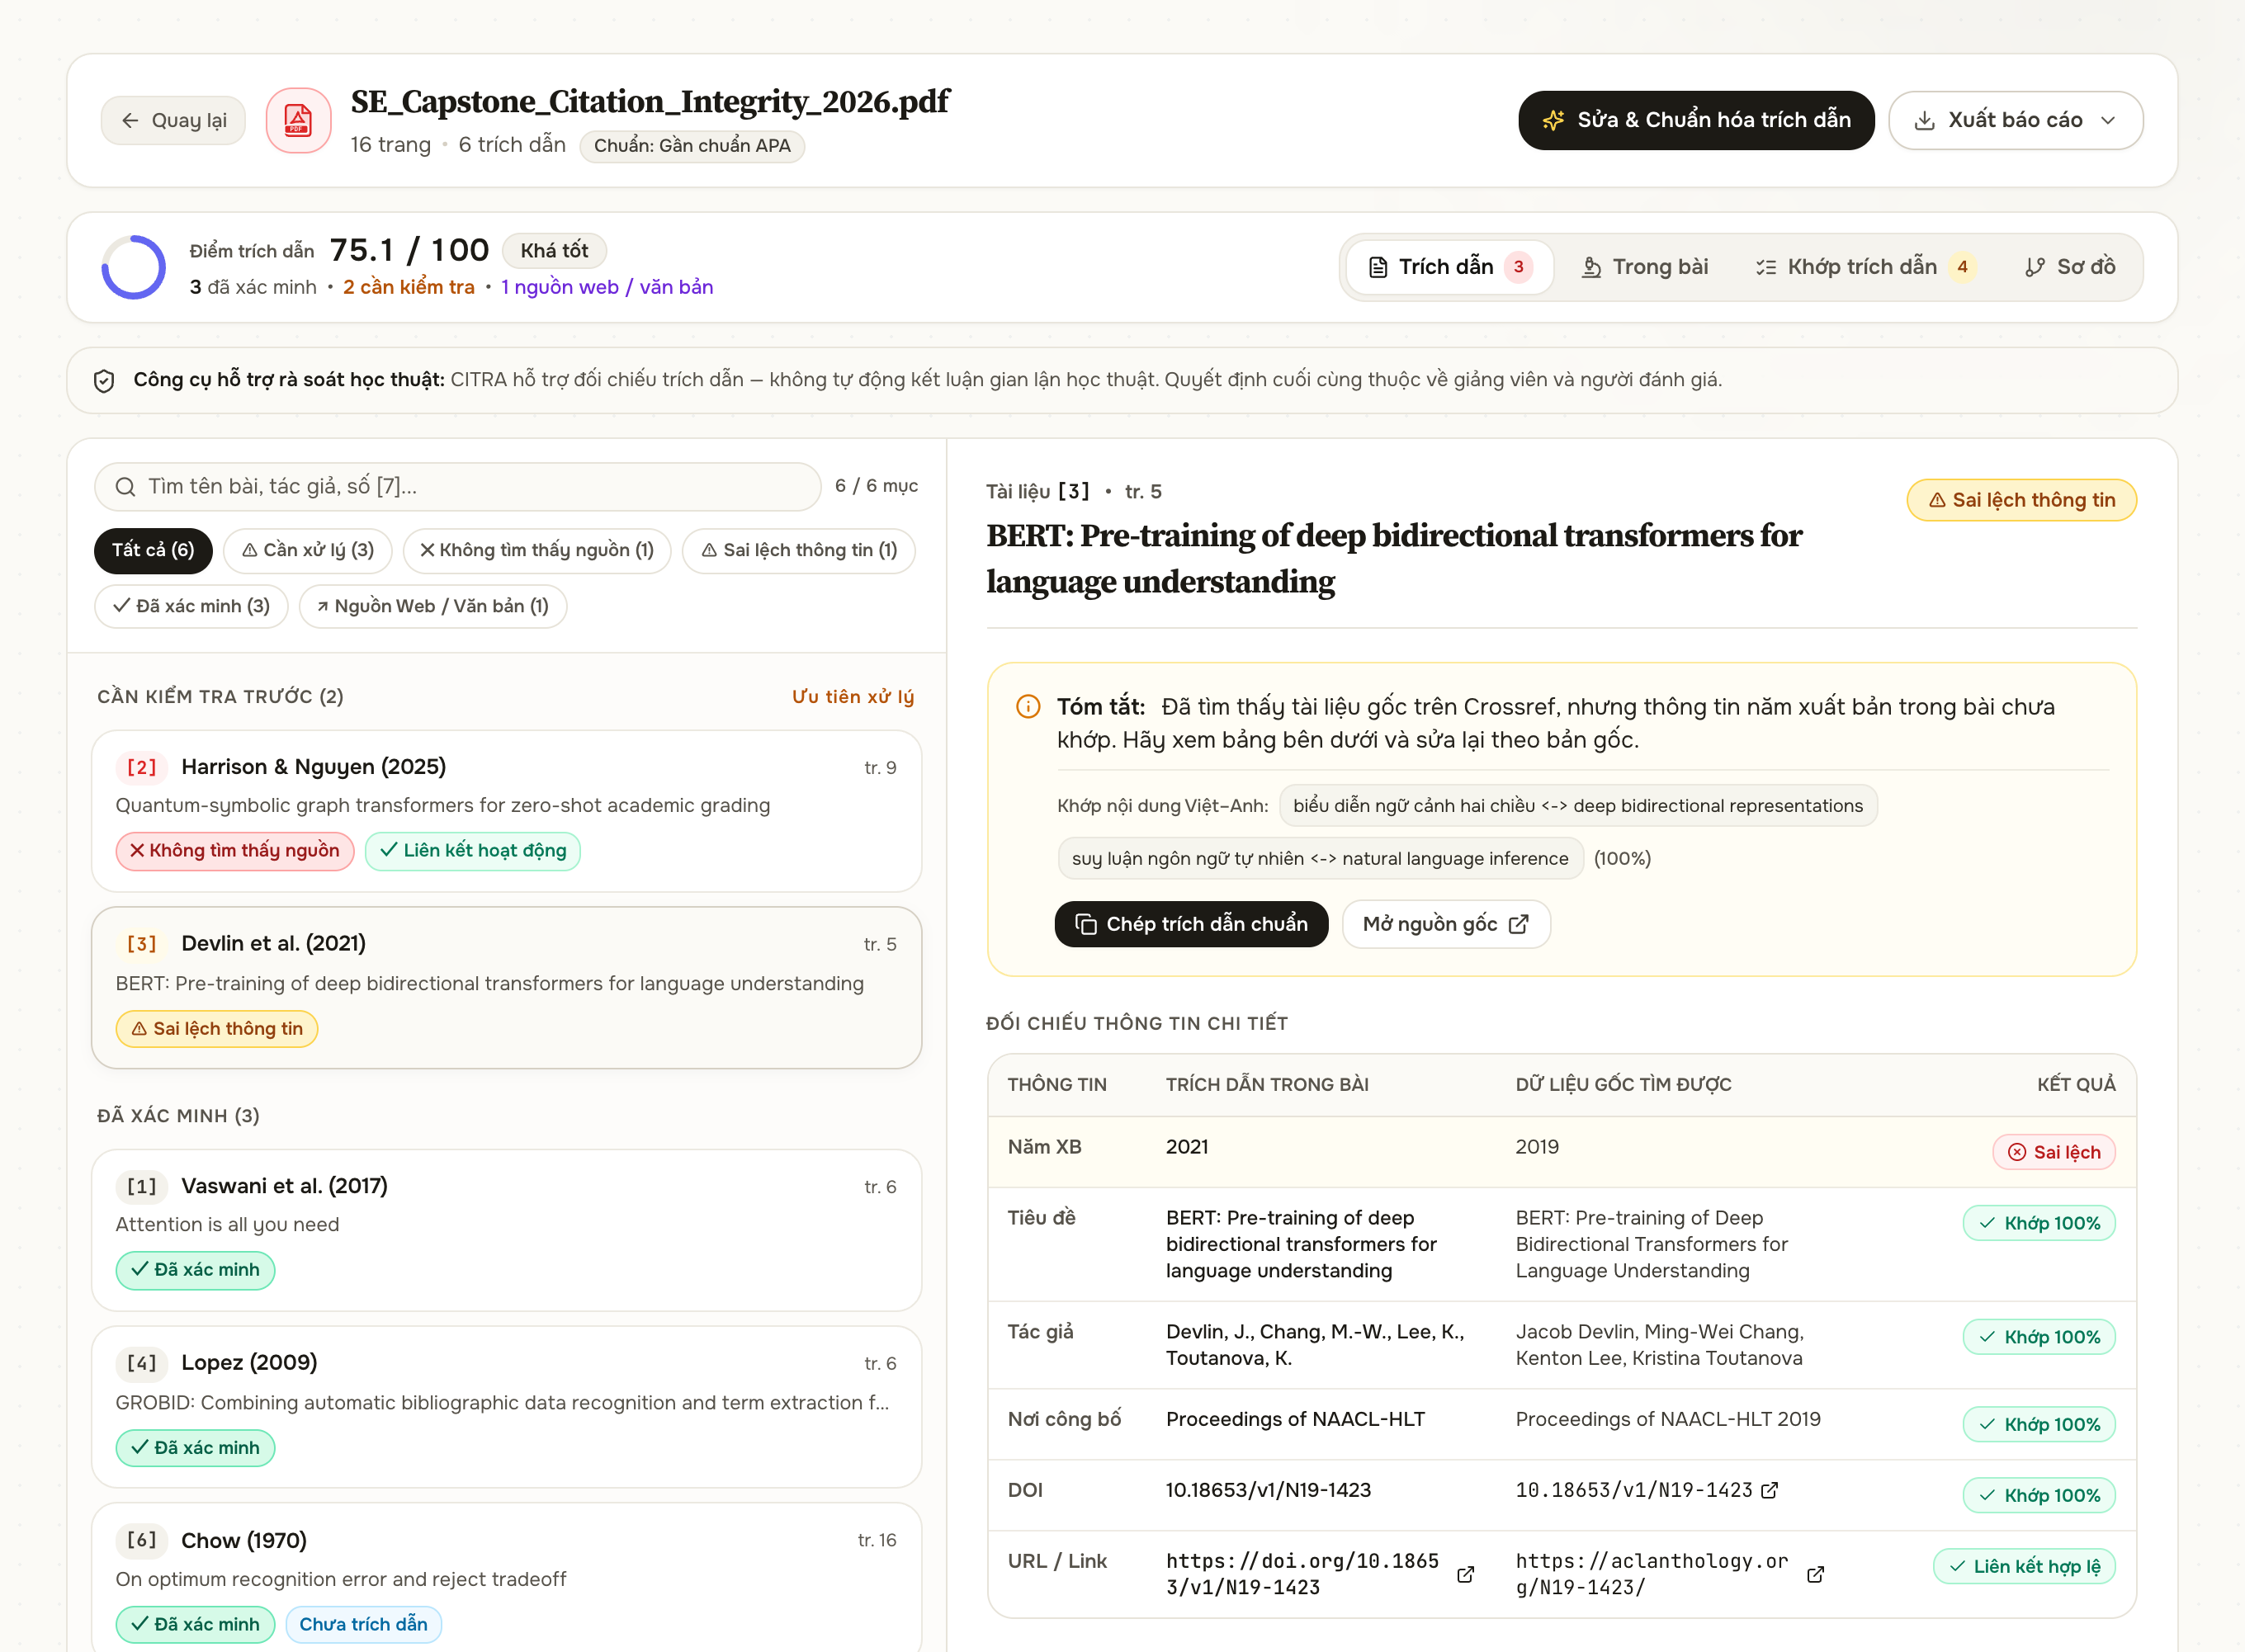
\includegraphics[width=0.94\textwidth,keepaspectratio]{picture/figures/06-reference-inspector.png}}
    \caption[Trình kiểm tra tài liệu tham khảo đối chiếu DOI lai ghép và sai lệch năm xuất bản]{Giao diện Kiểm tra tài liệu tham khảo trên bộ mẫu đồ án ($\text{CIS} = 75.1/100$, chính xác $75.08$), cô lập cảnh báo \texttt{suspected\_hallucination} dùng DOI lai ghép đối chiếu bản ghi AlphaFold2 gốc (trên) và lỗi \texttt{metadata\_error} lệch năm (\texttt{2021} so với \texttt{2019}, dưới).}
    \label{fig:demo-debugger}
\end{figure}

\begin{figure}[!htbp]
    \centering
    \fboxsep=0pt\fboxrule=0.4pt\fbox{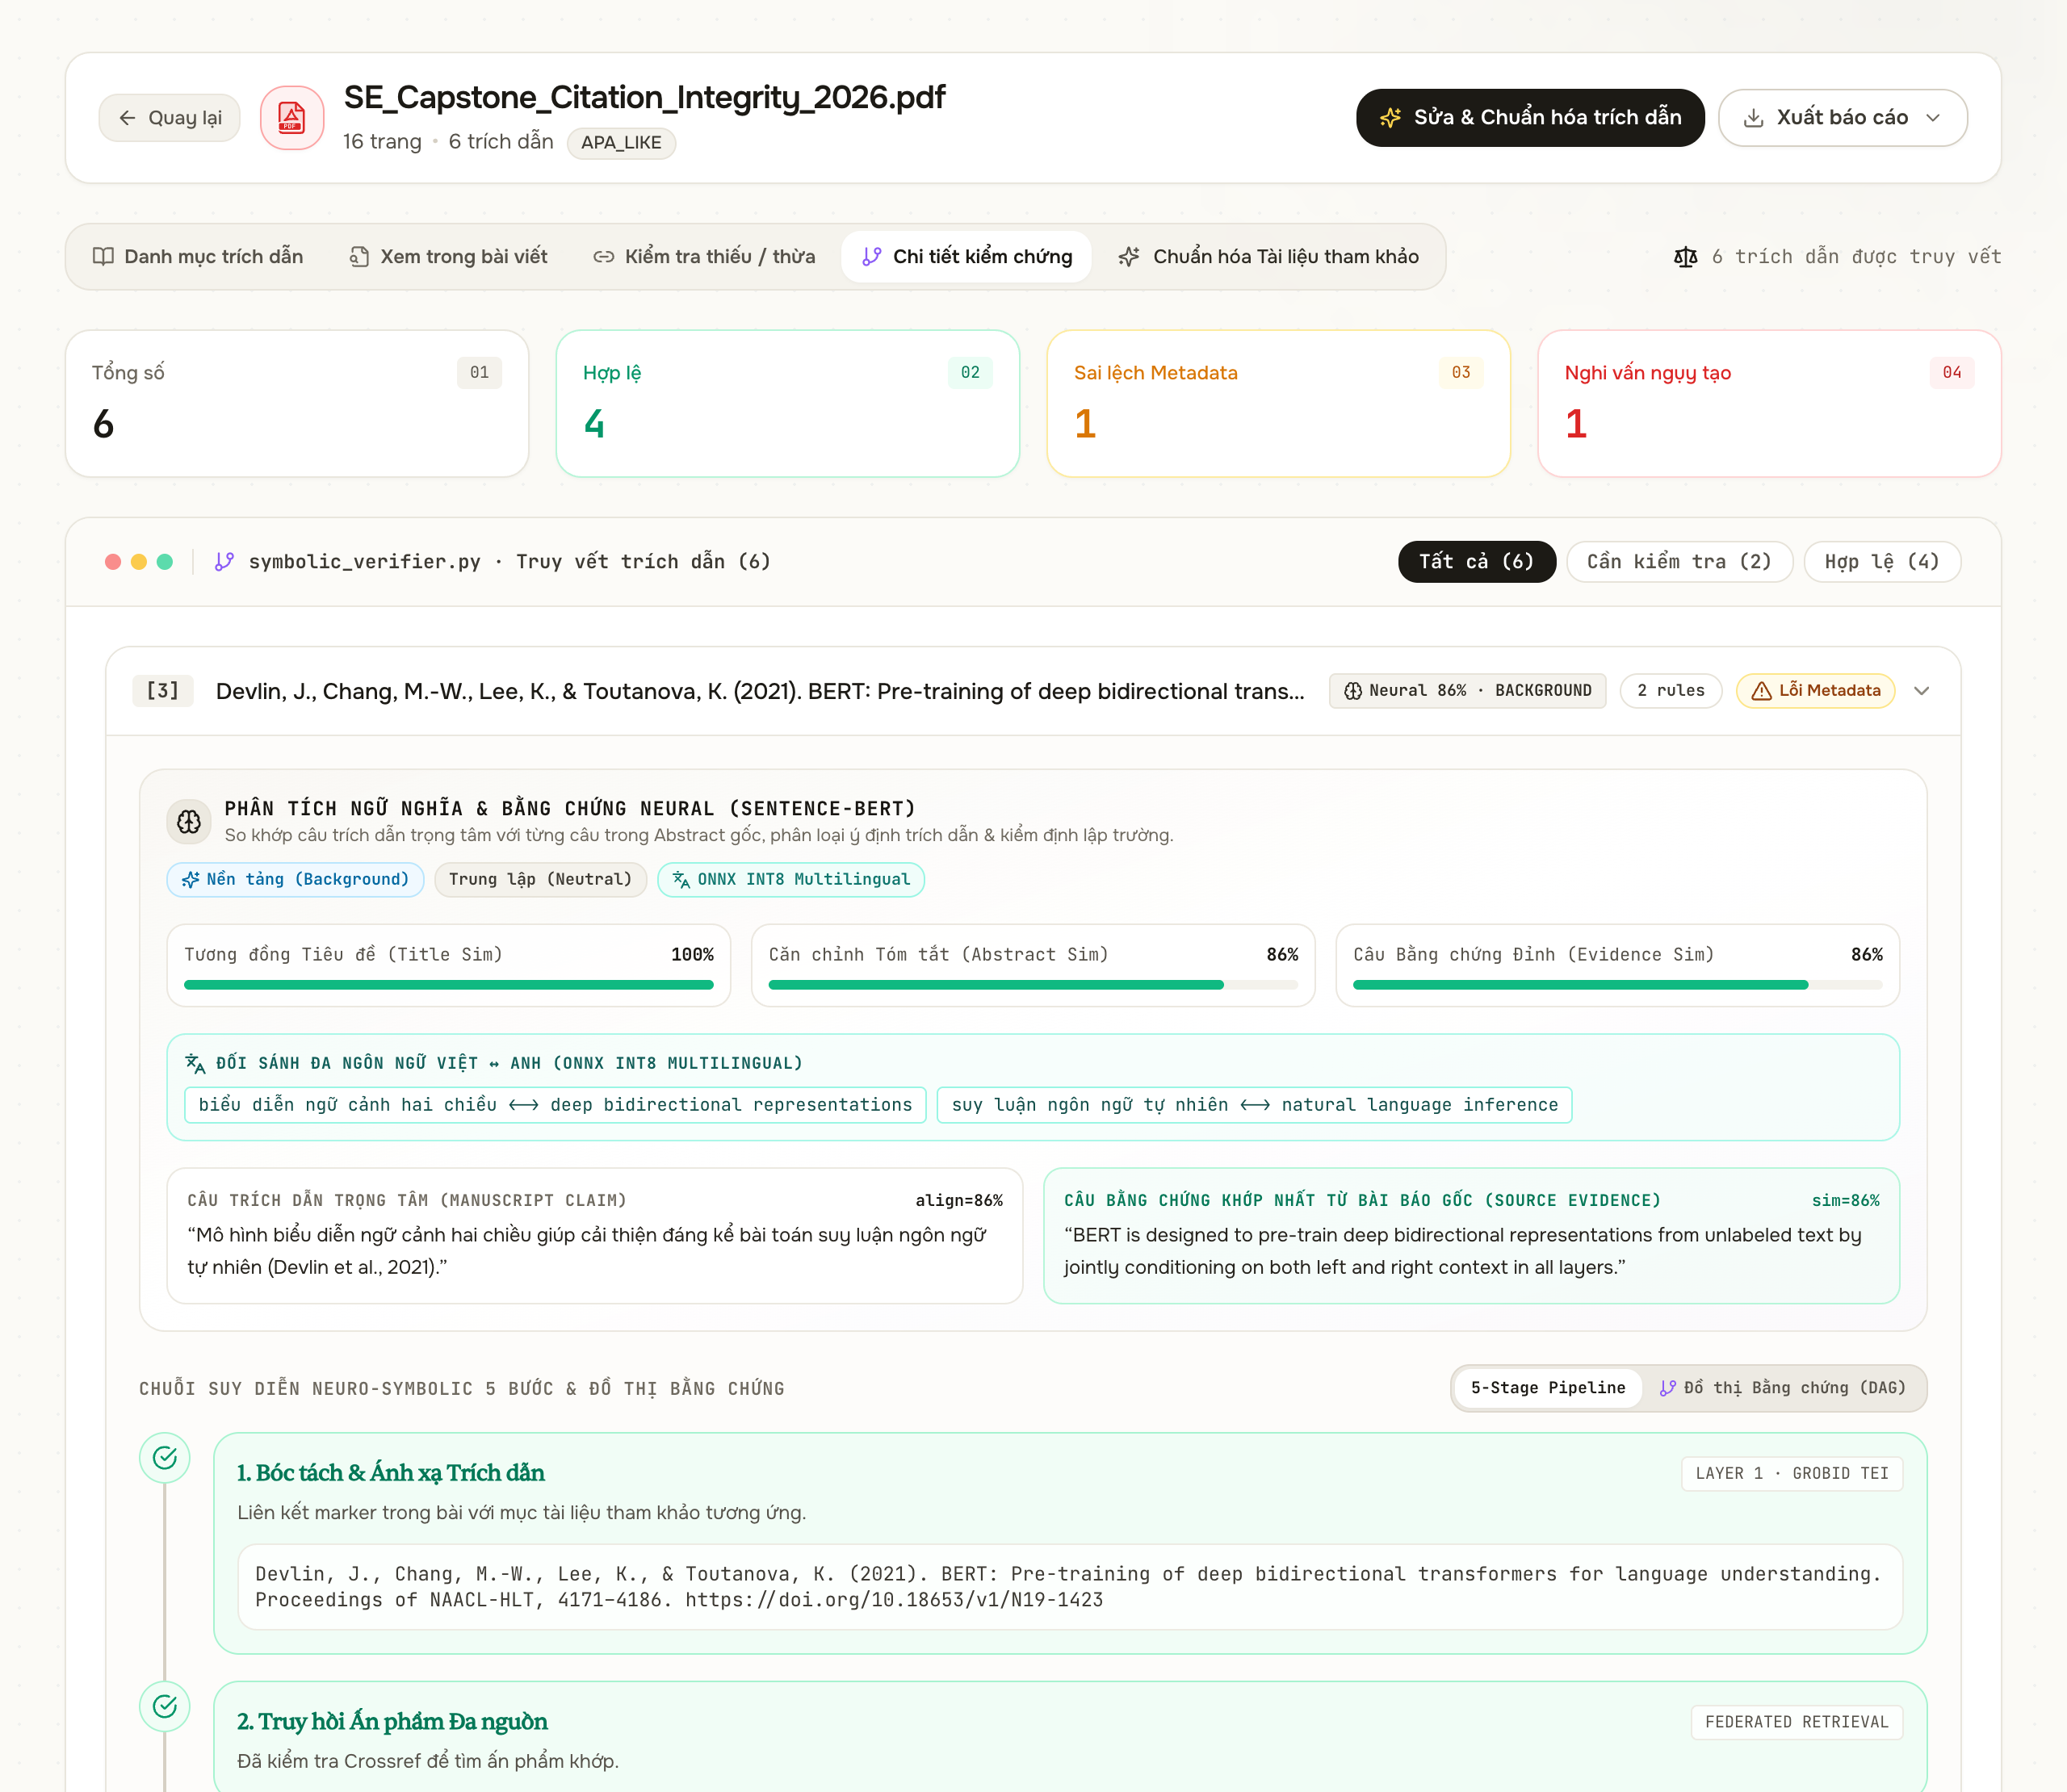
\includegraphics[width=0.94\textwidth,height=0.40\textheight,keepaspectratio]{picture/figures/07-logic-trace.png}}\\[6pt]
    \fboxsep=0pt\fboxrule=0.4pt\fbox{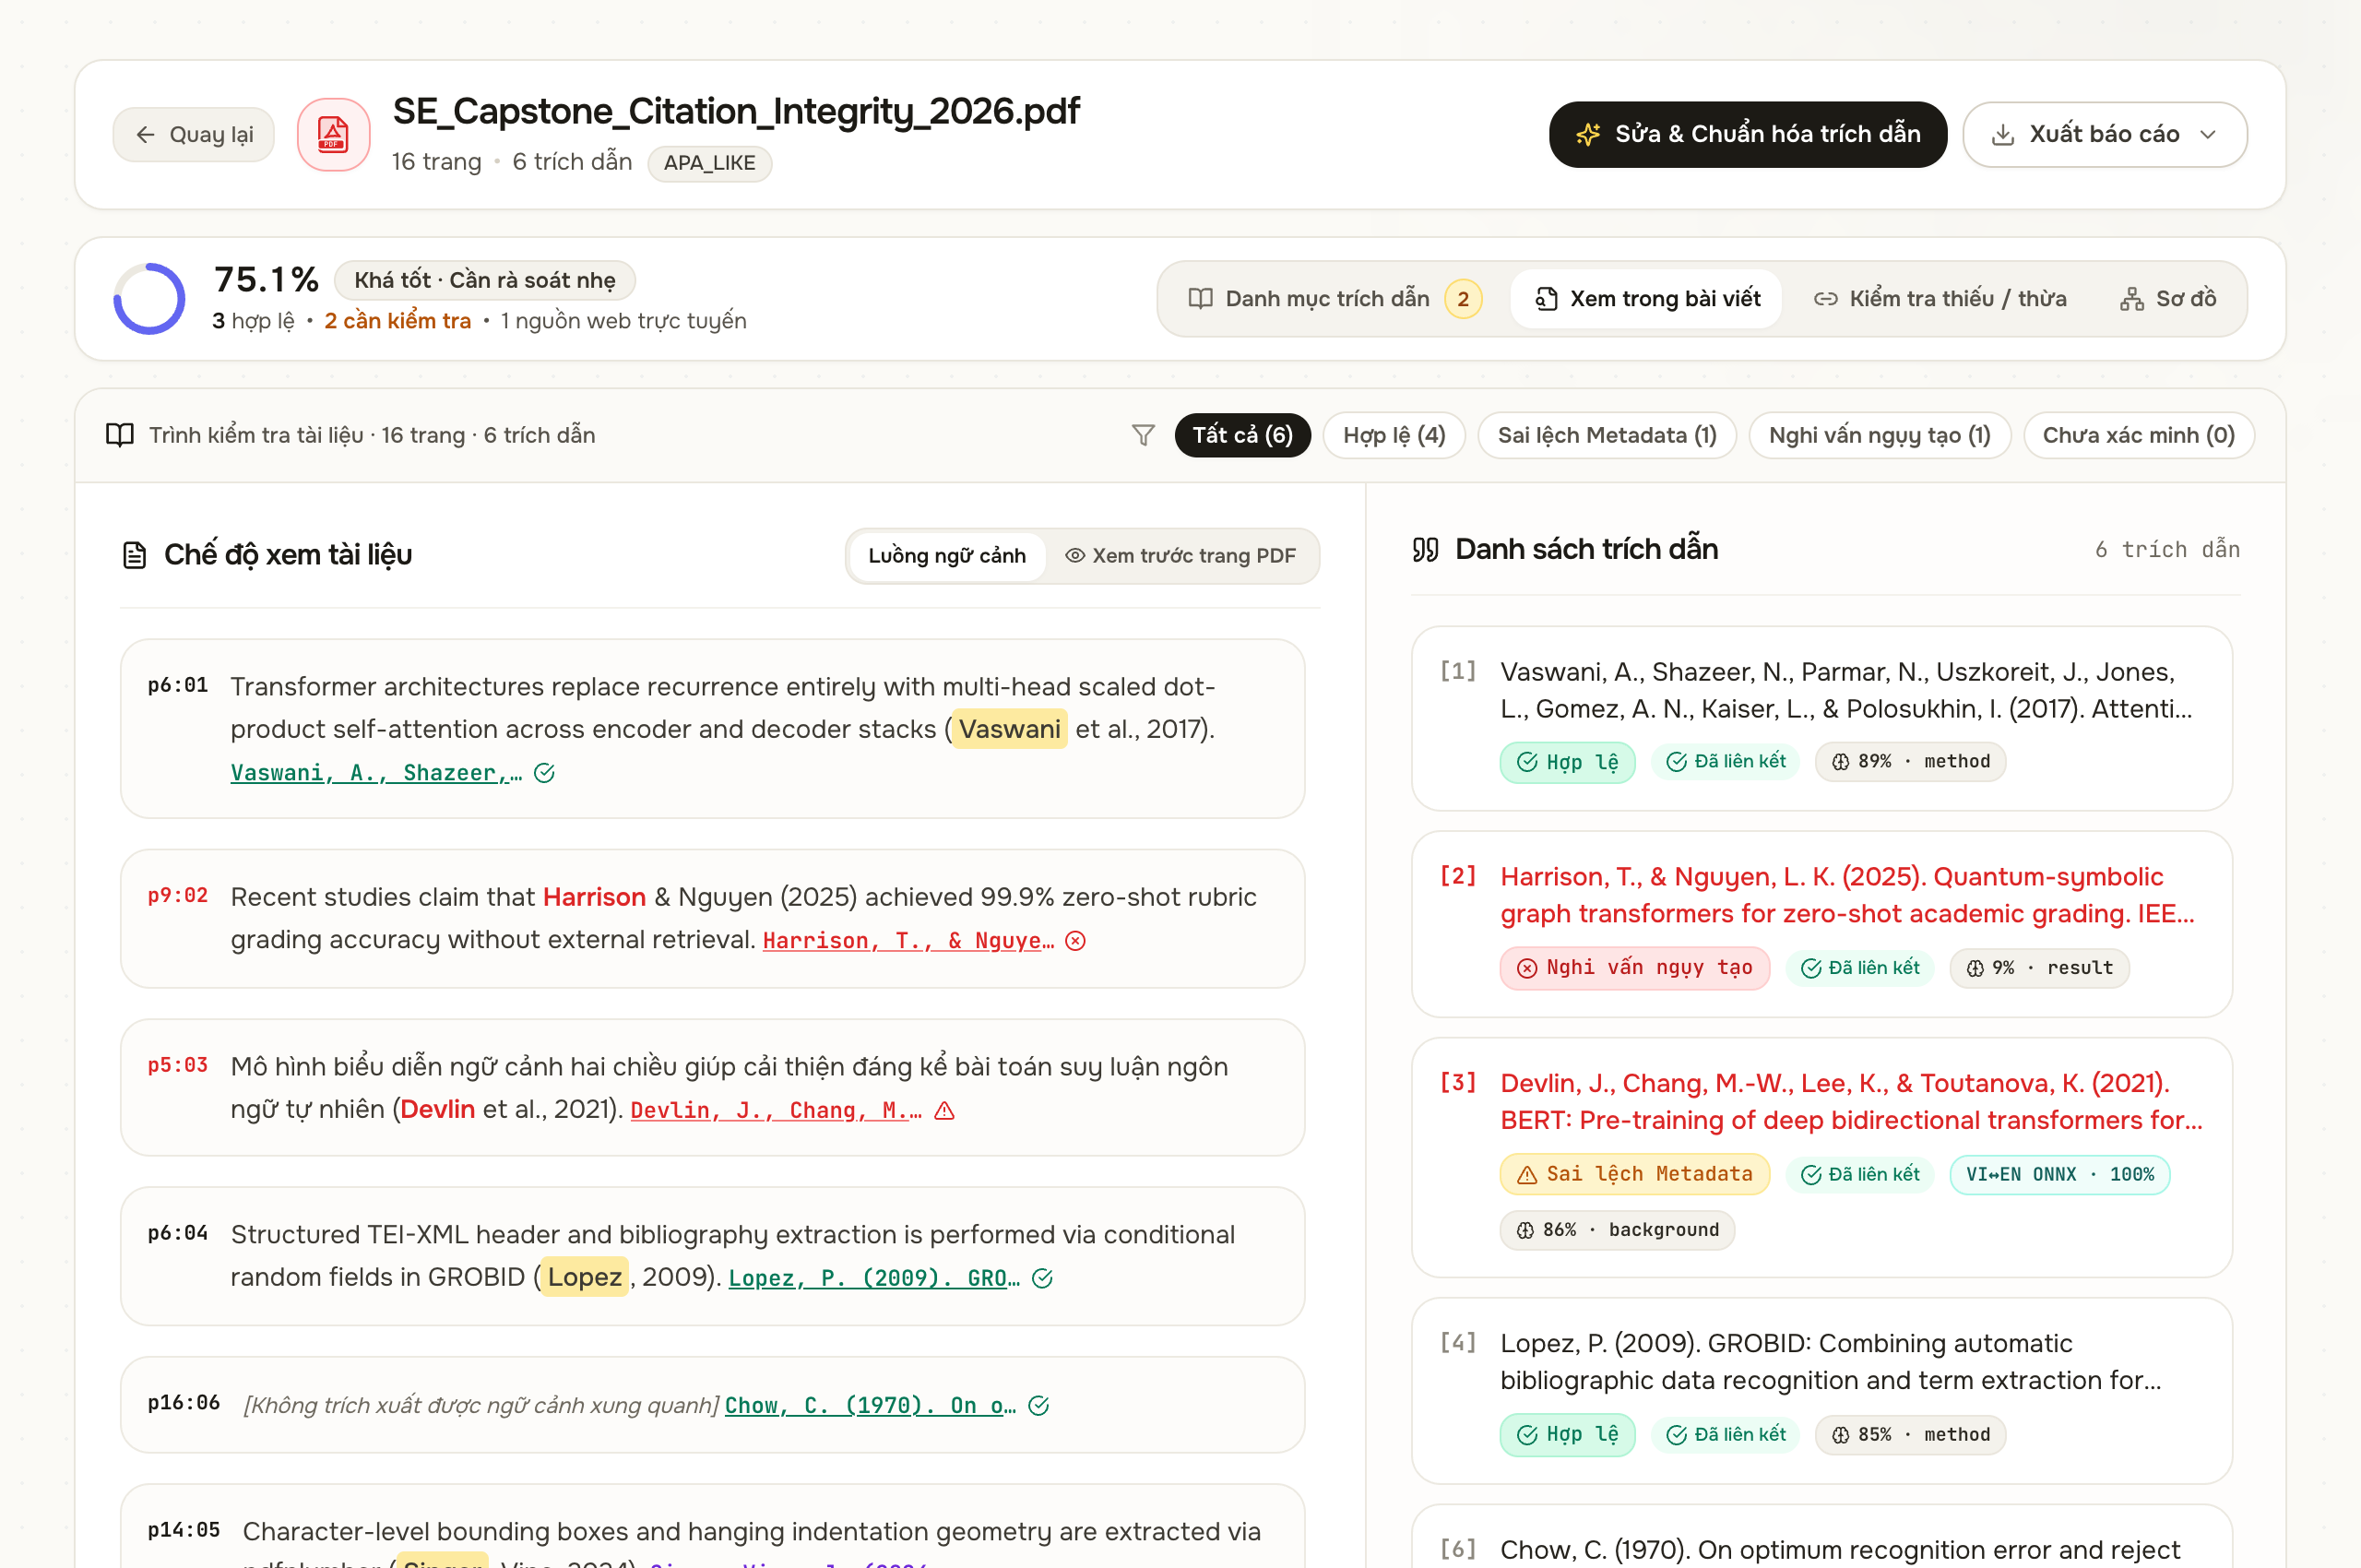
\includegraphics[width=0.94\textwidth,height=0.40\textheight,keepaspectratio]{picture/figures/09-document-inspector.png}}
    \caption[Vết suy diễn Logic Trace 5 bước song ngữ và Trình kiểm tra tài liệu trực tiếp]{Tiêu đề Logic Trace 5 giai đoạn kèm các bước đầu mở rộng hiển thị cầu nối khái niệm \texttt{VI}$\leftrightarrow$\texttt{EN} ONNX INT8 (trên) và luồng ngữ cảnh trực tiếp trong Trình kiểm tra tài liệu (dưới).}
    \label{fig:demo-trace-context}
\end{figure}

\begin{figure}[!htbp]
    \centering
    \fboxsep=0pt\fboxrule=0.4pt\fbox{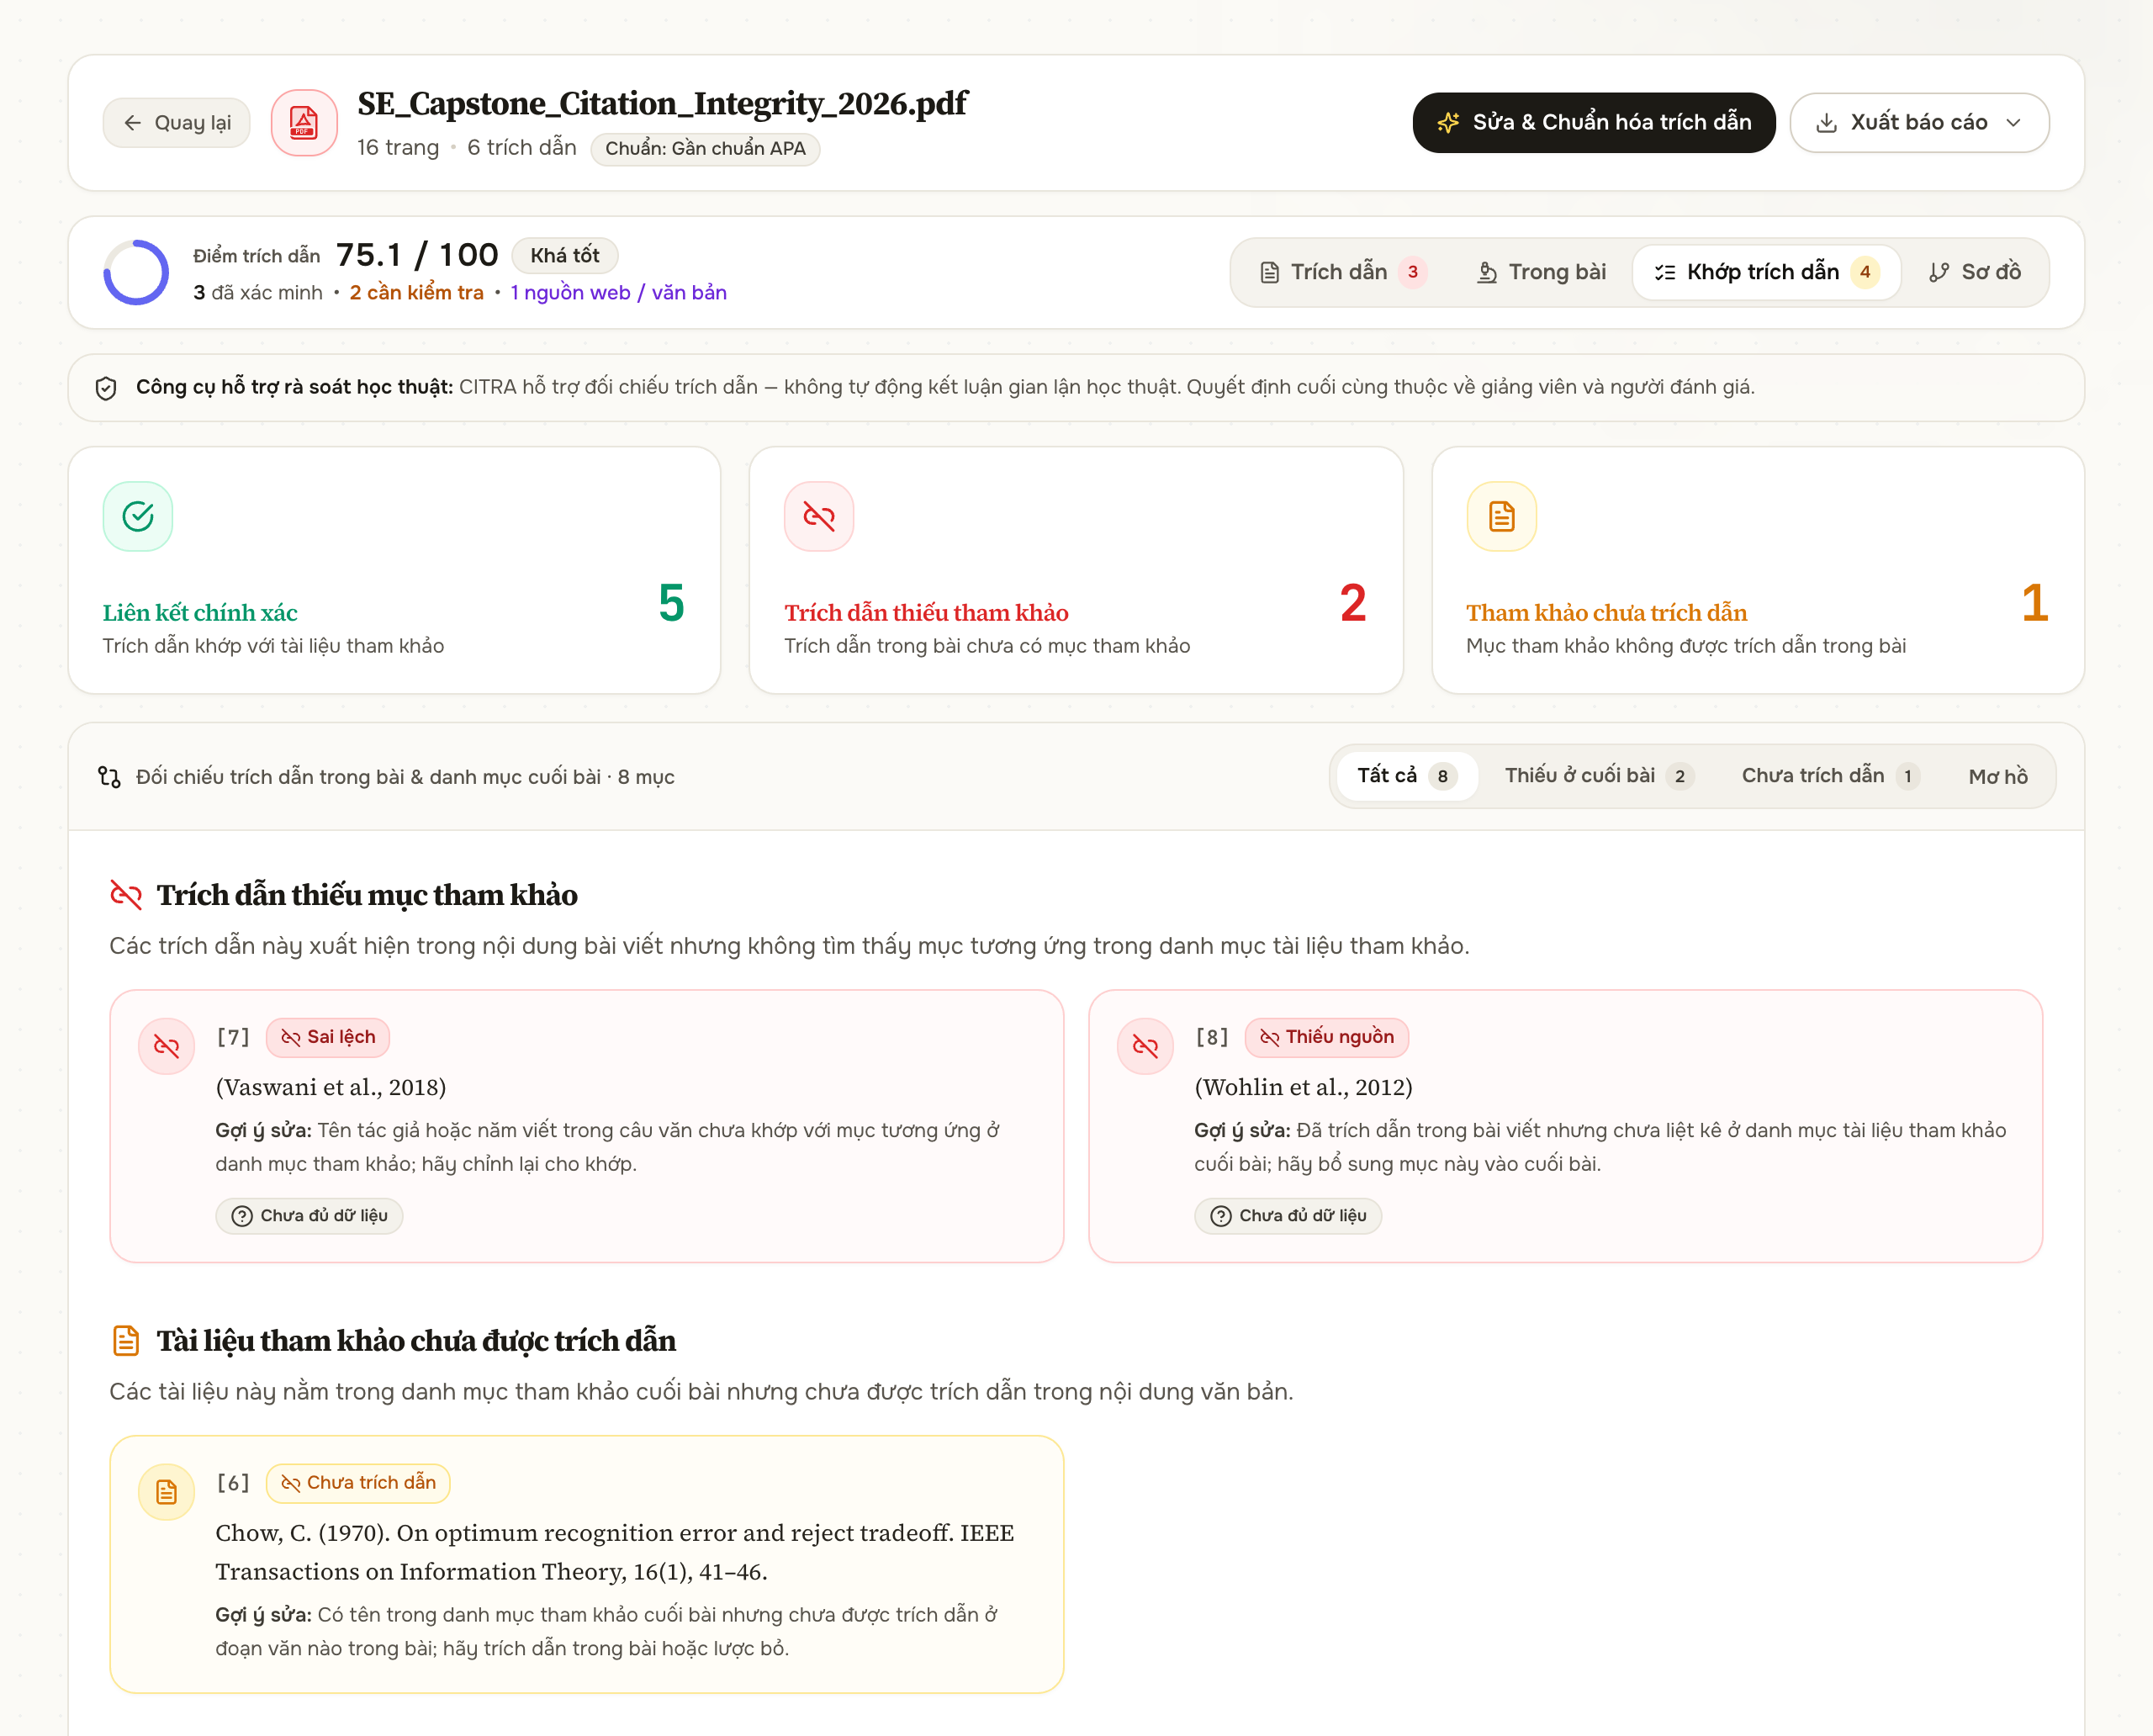
\includegraphics[width=0.96\textwidth,keepaspectratio]{picture/figures/08-consistency-check.png}}
    \caption[Kiểm tra tính nhất quán hai chiều cô lập trích dẫn mồ côi và mục chưa trích dẫn]{Giao diện Kiểm tra tính nhất quán hai chiều (\texttt{/verification/report/\{id\}/consistency}) tách bạch liên kết hợp lệ khỏi dấu trích dẫn mồ côi và tài liệu tham khảo chưa trích dẫn.}
    \label{fig:demo-consistency}
\end{figure}

\rqanswer{RQ4}{CITRA đạt độ chính xác 5 lớp $89.17\%$ (F1 hợp lệ $98.36\%$, chuẩn xác $100.00\%$, 0 cáo buộc sai trên bài thật) khi chạy trực tuyến 15 API trên 120 tài liệu tham khảo thô đa ngành ($100.00\%$ ngoại tuyến), nhận diện $97.7\%$--$100.0\%$ danh mục trên 310 PDF ($70.1\%$--$96.9\%$ liên kết thuần PyMuPDF) và đồng nhất $100\%$ ở chế độ API trực tuyến thuần trên các bản thảo thực tế.}

\section{RQ5: Độ trễ, hiệu quả bộ nhớ đệm và khả năng mở rộng đồng thời}
\label{sec:nfr-benchmarks}

Các bài đo phi chức năng cục bộ (Bảng~\ref{tab:nfr-step-latency}--\ref{tab:nfr-deadline-stress} và Hình~\ref{fig:nfr-scalability}) được chạy trên phần cứng Apple Silicon ARM64 (\texttt{macOS 26.6.2}, Python \texttt{3.14.6}, thuần CPU, bật Sentence-BERT thật) qua \texttt{scripts/benchmark\_pipeline\_performance.py}, còn Bảng~\ref{tab:nfr-grobid-prod} đo trực tiếp container trên máy chủ ảo Google Compute Engine 2 vCPU, $5.8\text{\,GiB}$ RAM (\texttt{e2-custom-medium-6144}).

Độ trễ $P_{90}$ ở bộ đệm ấm trên $n = 5$ lượt đo liên tục (sau 1 lượt làm nóng; lưu ý $P_{99}$ với $n = 5$ phản ánh giá trị cực đại quan sát) tăng tuyến tính từ $0.58\text{\,s}$ (bài báo 12 trang) lên $1.33\text{\,s}$ (đồ án 50 trang, đạt tốt ngưỡng $2.5\text{\,s}$ của \texttt{NFR-01}) và $4.22\text{\,s}$ (chuyên khảo 156 trang), với RSS API tối đa $1{,}030.8\text{\,MB}$ ($\le 1.5\text{\,GB}$ \texttt{NFR-02}) và đỉnh tăng heap cực đại từng chặng ở $11.10\text{\,MB}$ ($\le 25\text{\,MB}$).

Để kiểm chứng trực tiếp SLA mạng WAN lạnh của \texttt{NFR-01} trên đúng quy mô đồ án 50 trang, Bảng~\ref{tab:nfr-cold-warm-cache} báo cáo \emph{cả} bài báo 12 trang ($n = 1$: $9.41\text{\,s}$ lạnh $\rightarrow 0.48\text{\,s}$ ấm, tăng tốc truy hồi $688.72\times$) \emph{lẫn} phép đo mới $n = 3$ tiến trình cô lập trên mạng WAN lạnh đối với \textbf{đồ án tốt nghiệp 50 trang} (\texttt{20-theses/109.pdf}, 32/32 truy vấn trực tiếp Crossref+OpenAlex, PyMuPDF + SBERT thật): trung vị độ trễ mạng WAN lạnh đạt \textbf{12.64\,s} ($12{,}639.1\text{\,ms} \le 15\text{\,s}$, đạt \texttt{NFR-01}; chặng truy hồi $10{,}687.8\text{\,ms}$), rút xuống \textbf{2.00\,s} khi ấm bộ đệm (tăng tốc truy hồi \textbf{151.2$\times$}, tổng thể \textbf{6.31$\times$}). Chênh lệch $0.70\text{\,s}$ giữa trung vị ấm $2.00\text{\,s}$ tại Bảng~\ref{tab:nfr-cold-warm-cache} và trung bình $1.31\text{\,s}$ ($P_{90} = 1.33\text{\,s}$) tại Bảng~\ref{tab:nfr-step-latency} xuất phát từ việc khởi chạy tiến trình mới cô lập với đệm trang hệ điều hành nguội cho PyMuPDF/SQLite so với vòng lặp làm nóng liên tục trong cùng tiến trình.

\begin{figure}[!htbp]
    \centering
    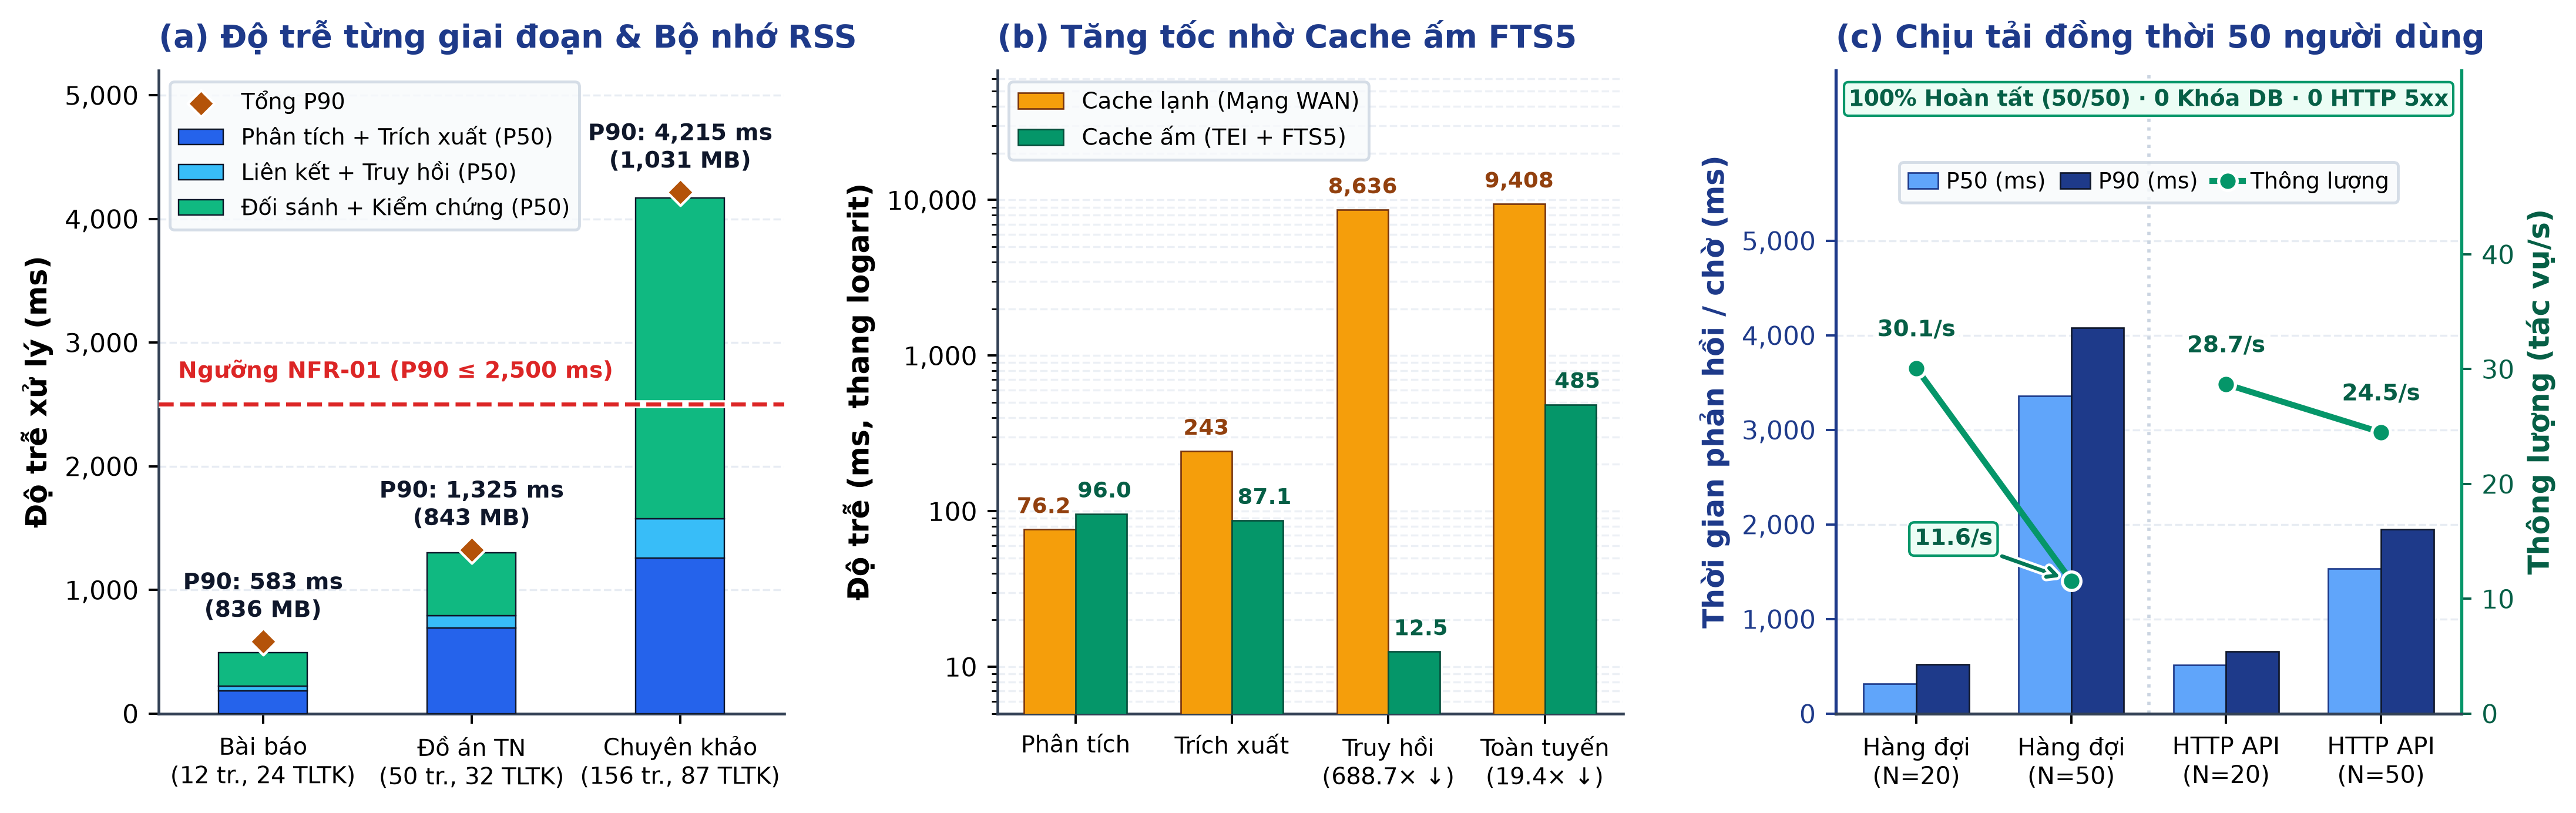
\includegraphics[width=\textwidth,keepaspectratio]{picture/figures/fig5_2_nfr_scalability.png}
    \caption[Độ trễ từng chặng, tăng tốc bộ nhớ đệm thang log và kiểm thử tải đồng thời 50 người dùng]{Các biểu đồ hiệu năng và khả năng mở rộng: (a)~độ trễ bộ đệm ấm cộng tính theo chặng và RSS so với SLA \texttt{NFR-01}, (b)~so sánh WAN lạnh và bộ đệm ấm theo thang log trên bài báo 12 trang và đồ án 50 trang ($12.64\text{\,s} \le 15\text{\,s}$), và (c)~kiểm thử tải I/O, hàng đợi và SQLite WAL với 20 và 50 người dùng (NLP giả lập).}
    \label{fig:nfr-scalability}
\end{figure}

{\setlength{\tabcolsep}{3.0pt}
\begin{table}[!htbp]
\centering
\caption{Trung bình độ trễ cộng tính theo chặng, phân vị tổng ($n = 5$ sau 1 lượt làm nóng, Apple ARM64 CPU) và mức dùng RAM trên ba quy mô bản thảo.}\label{tab:nfr-step-latency}
\begin{tabular}{|L{0.21}|L{0.23}|C{0.11}|C{0.15}|C{0.10}|C{0.10}|C{0.10}|}
\hline
\textbf{Quy mô bản thảo} & \textbf{Nhóm chặng} & \textbf{TB (ms)} & \textbf{$P_{50} / P_{90}$ (ms)} & \textbf{$P_{99}$\textsuperscript{*} (ms)} & \textbf{Đỉnh $\Delta$ (MB)} & \textbf{RSS (MB)} \\
\hline
\textbf{Bài báo} (12\,tr., 24\,TLTK) & Phân tích + chuẩn + trích & 209.7 & --- & --- & 1.61 & 835.7 \\
 & Liên kết + truy hồi & 42.0 & --- & --- & 0.16 & 835.7 \\
 & Đối sánh + kiểm + chấm & 268.9 & --- & --- & 0.16 & 835.7 \\
 & \textbf{Tổng (Cả 8 bước)} & \textbf{520.5} & \textbf{494.1 / 583.4} & \textbf{635.5} & \textbf{1.61} & \textbf{835.7} \\
\hline
\textbf{Đồ án} (50\,tr., 32\,TLTK) & Phân tích + chuẩn + trích & 696.9 & --- & --- & 4.39 & 843.4 \\
 & Liên kết + truy hồi & 98.2 & --- & --- & 0.26 & 843.4 \\
 & Đối sánh + kiểm + chấm & 513.3 & --- & --- & 0.22 & 843.4 \\
 & \textbf{Tổng (Cả 8 bước)} & \textbf{1308.4} & \textbf{1306.9 / 1325.1} & \textbf{1333.0} & \textbf{4.39} & \textbf{843.4} \\
\hline
\textbf{Chuyên khảo} (156\,tr., 87\,TLTK) & Phân tích + chuẩn + trích & 1261.5 & --- & --- & 11.10 & 1030.8 \\
 & Liên kết + truy hồi & 317.3 & --- & --- & 0.24 & 1030.8 \\
 & Đối sánh + kiểm + chấm & 2577.6 & --- & --- & 1.16 & 1030.8 \\
 & \textbf{Tổng (Cả 8 bước)} & \textbf{4156.5} & \textbf{4159.7 / 4215.3} & \textbf{4215.6} & \textbf{11.10} & \textbf{1030.8} \\
\hline
\multicolumn{7}{p{\dimexpr\textwidth-2\tabcolsep\relax}}{\scriptsize\textsuperscript{*}Trung bình (TB) các nhóm chặng cộng tính nghiêm ngặt bằng TB Tổng ($\pm 0.1\text{\,ms}$ làm tròn; độ lệch chuẩn SD: $67.7$, $16.8$ và $66.6\text{\,ms}$). Các phân vị không cộng tính theo nhóm chặng nên báo cáo trên Tổng ($P_{99}$ với $n=5$ xấp xỉ cực đại mẫu). Cột Đỉnh $\Delta$ lấy cực đại (\texttt{max}) qua các bước con.}
\end{tabular}
\end{table}
}

{\setlength{\tabcolsep}{3.5pt}
\begin{table}[!htbp]
\centering
\caption{So sánh độ trễ WAN lạnh và bộ nhớ đệm ấm trên bài báo 12 trang và báo cáo đồ án 50 trang.}\label{tab:nfr-cold-warm-cache}
\begin{tabular}{|L{0.29}|C{0.11}|C{0.11}|C{0.13}|C{0.13}|C{0.12}|C{0.11}|}
\hline
\textbf{Tài liệu \& Chế độ đệm} & \textbf{Phân tích (ms)} & \textbf{Trích xuất (ms)} & \textbf{Truy hồi (ms)} & \textbf{Tổng (ms)} & \textbf{Tăng tốc truy hồi} & \textbf{Tăng tốc E2E} \\
\hline
Bài báo 12\,tr.\ --- WAN lạnh ($n=1$) & 76.2 & 243.1 & 8,635.8 & 9,407.6 & $1.00\times$ & $1.00\times$ \\
\hline
\textbf{Bài báo 12\,tr.\ --- Đệm ấm} & 96.0 & \textbf{87.1} & \textbf{12.54}\textsuperscript{*} & \textbf{484.8} & \textbf{$688.72\times$} & \textbf{$19.41\times$} \\
\hline
Đồ án 50\,tr.\ --- WAN lạnh ($n=3$, trung vị) & 453.3 & 732.6 & 10,687.8 & \textbf{12,639.1} & $1.00\times$ & $1.00\times$ \\
\hline
\textbf{Đồ án 50\,tr.\ --- Đệm ấm} ($n=3$)\textsuperscript{$\dagger$} & 452.1 & 730.6 & \textbf{70.7} & \textbf{2,003.9} & \textbf{$151.2\times$} & \textbf{$6.31\times$} \\
\hline
\multicolumn{7}{p{\dimexpr\textwidth-2\tabcolsep\relax}}{\scriptsize\textsuperscript{*}Hệ số $688.72\times$ tính từ độ trễ chưa làm tròn ($12.539\text{\,ms}$). \textsuperscript{$\dagger$}Lượt ấm tiến trình cô lập (trung vị $2.00\text{\,s}$) gồm đệm trang HĐH nguội so với vòng lặp ấm liên tục ($1.31\text{\,s}$ TB / $1.33\text{\,s}$ $P_{90}$) tại Bảng~\ref{tab:nfr-step-latency}.}
\end{tabular}
\end{table}
}

Bảng~\ref{tab:nfr-deadline-stress} cô lập kiểm thử \textbf{tầng tải lên HTTP multipart, kế toán hạn mức CAS, ghi đồng thời SQLite WAL và hàng đợi FIFO \texttt{Pipeline\allowbreak{}Admission\allowbreak{}Controller}} dưới tải đột biến 20 và 50 sinh viên trên tệp PDF mẫu 2 trang / 3 trích dẫn với \textbf{tầng NLP giả lập (stubbed)} nhằm tạo áp lực tối đa lên khóa CSDL và lập lịch hàng đợi. Toàn bộ $50/50$ lượt nộp hoàn tất với $0$ lỗi khóa SQLite và $0$ lỗi HTTP 5xx/429 ($11.57\text{\,bài/s}$ qua hàng đợi; $24.49\text{\,req/s}$ tiếp nhận HTTP). Theo định luật Little, khi chạy đủ AI trên CPU (\texttt{max\_concurrent=3}, $1.31$--$2.00\text{\,s}$ đệm ấm / $12.64\text{\,s}$ WAN lạnh mỗi đồ án 50 trang), thông lượng kiểm chứng thực tế đạt khoảng $\sim 1.5$--$2.3\text{\,bài/s}$ (đệm ấm) hoặc $\sim 0.24\text{\,bài/s}$ (WAN lạnh), còn hàng đợi điều phối hấp thụ êm toàn bộ 50 lượt nộp mà không từ chối yêu cầu.

{\setlength{\tabcolsep}{3pt}
\begin{table}[!htbp]
\centering
\caption{Kiểm thử chịu tải I/O, hàng đợi điều phối và ghi đồng thời SQLite WAL (tầng NLP giả lập, PDF 2 trang).}\label{tab:nfr-deadline-stress}
\begin{tabular}{|L{0.23}|C{0.07}|C{0.15}|C{0.21}|C{0.19}|C{0.15}|}
\hline
\textbf{Kịch bản tải (NLP giả lập)} & \textbf{$N$} & \textbf{Hoàn tất} & \textbf{Tải lên / Hàng đợi $P_{50}/P_{90}$ (ms)} & \textbf{Thông lượng} & \textbf{Khóa CSDL / 5xx} \\
\hline
Hàng đợi điều phối & 20 & \textbf{20 / 20} & 315.5 / 520.7 & \textbf{30.07 bài/s} & \textbf{0 / 0} \\
\hline
Hàng đợi điều phối & \textbf{50} & \textbf{50 / 50} & 3361.1 / 4079.2 & 11.57 bài/s & \textbf{0 / 0} \\
\hline
HTTP \texttt{POST /\allowbreak api/\allowbreak essays} & 20 & \textbf{20 / 20} & 514.2 / 659.4 & \textbf{28.68 req/s} & \textbf{0 / 0} \\
\hline
HTTP \texttt{POST /\allowbreak api/\allowbreak essays} & \textbf{50} & \textbf{50 / 50} & 1530.2 / 1948.0 & 24.49 req/s & \textbf{0 / 0} \\
\hline
\end{tabular}
\end{table}
}

Để xác minh hành vi bộ nhớ thực tế trên máy chủ vận hành với bản thảo dài khi tắt đệm đĩa, Bảng~\ref{tab:nfr-grobid-prod} đối chiếu container GROBID $3\text{\,GiB}$ cũ (\texttt{-Xmx1280m}, \texttt{concurrency=10}, bật \texttt{teiCoordinates}) với cấu hình tối ưu $4\text{\,GiB}$ (\texttt{-Xmx768m}, \texttt{concurrency=2}, \texttt{pdfalto=1024\,MB}, tắt \texttt{teiCoordinates}) trên máy chủ GCE bằng bản thảo 117 trang ($10.63\text{\,MB}$) của chính báo cáo này. Cấp bộ nhớ vượt ngưỡng $3.1\text{\,GiB}$ của mô hình Wapiti gốc xóa sạch swap ($2.19\text{\,GiB} \rightarrow 0\text{\,B}$), giảm $99.74\%$ lỗi trang cứng ($91{,}718 \rightarrow 239$ nền khởi động với $+0$ tăng thêm khi chạy), tăng tốc GROBID không đệm $5.48\times$ ở lượt ấm ($95.53\text{\,s} \rightarrow 17.44\text{\,s}$) và xử lý đồng thời hai luận văn 117 trang trong $31.31\text{\,s}$ trong khi còn dư $885\text{\,MiB}$ RAM. Các yêu cầu phi chức năng còn lại đều đạt định lượng: \texttt{NFR-07} đạt WCAG 2.1 AA và $0\text{\,px}$ tràn lề trên 5 khung nhìn; \texttt{NFR-08} biên dịch gói khởi động $231.50\text{\,kB}$ ($67.50\text{\,kB}$ nén gzip $\le 250\text{\,kB}$); \texttt{NFR-09} chạy $3{,}110$ kiểm tra tự động mặc định ($3{,}119$ tổng, $0$ lỗi); và \texttt{NFR-10} khởi động đủ 3 container trong $\le 60\text{\,s}$ ấm ($\le 120\text{\,s}$ nạp mô hình lạnh) với $0$ phụ thuộc GPU.

{\setlength{\tabcolsep}{3.5pt}
\begin{table}[!htbp]
\centering
\caption{Đo kiểm thực tế trên máy chủ GCE vận hành đối với GROBID không đệm trên bản thảo luận văn 117 trang ($10.63\text{\,MB}$) trước và sau tối ưu.}\label{tab:nfr-grobid-prod}
\begin{tabular}{|L{0.28}|C{0.15}|C{0.13}|C{0.16}|C{0.13}|C{0.15}|}
\hline
\textbf{Cấu hình vận hành} & \textbf{Thời gian GROBID} & \textbf{Đỉnh Swap} & \textbf{Lỗi trang cứng} & \textbf{Kích thước TEI} & \textbf{TLTK / Nội văn} \\
\hline
Cấu hình cũ \texttt{3G} (\texttt{-Xmx1280m}, pool 10) & 95.53\,s & 2.19\,GiB & 91,718 & 236.3\,kB & 46 / 73 \\
\hline
\textbf{Tối ưu \texttt{4G} --- JIT nguội (không đệm)} & \textbf{46.93\,s} ($2.04\times$) & \textbf{0\,B} & \textbf{239 (+0 chạy)} & \textbf{227.3\,kB} & \textbf{46 / 73} \\
\hline
\textbf{Tối ưu \texttt{4G} --- JIT ấm (không đệm)} & \textbf{17.44\,s} ($5.48\times$) & \textbf{0\,B} & \textbf{239 (+0 chạy)} & \textbf{227.3\,kB} & \textbf{46 / 73} \\
\hline
\textbf{Tối ưu \texttt{4G} --- 2$\times$ Song song (234\,tr.)} & \textbf{31.31\,s thực} & \textbf{0\,B} & \textbf{239 (+0 chạy)} & \textbf{227.3\,kB} & \textbf{46 / 73 ($\times 2$)} \\
\hline
\end{tabular}
\end{table}
}

\rqanswer{RQ5}{CITRA kiểm chứng đồ án 50 trang trong $1.33\text{\,s}$ ($P_{90}$ đệm ấm) và trung vị $12.64\text{\,s}$ WAN lạnh ($32/32$ truy vấn thực, đạt SLA $15\text{\,s}$ của \texttt{NFR-01}; tăng tốc truy hồi $151.2\times$), giới hạn RSS API ở $1.03\text{\,GB}$, triệt tiêu swap GROBID trên GCE ($95.53\text{\,s} \rightarrow 17.44\text{\,s}$, $0\text{\,B}$ swap), đáp ứng \texttt{NFR-07}--\texttt{NFR-10} và chịu tải I/O 50 người dùng đồng thời với $0$ lỗi khóa SQLite hay HTTP 5xx.}

\section{Các mối đe dọa đến độ giá trị thực nghiệm}
\label{sec:difficulties}

Theo khung phân loại của Wohlin và cộng sự~\cite{wohlin2012experimentation}, bốn nhóm mối đe dọa thực chất đối với độ giá trị thực nghiệm được phân tích thẳng thắn dưới đây.

\subsection{Độ giá trị nội tại}

Tập chuẩn 120,000 mẫu sinh biến thể nhiễu theo chương trình bám sát phân loại tầng kiểm chứng; do đó $99.67\%$ phản ánh \emph{tính nhất quán tầng quyết định có kiểm soát} chứ không thay thế độ chính xác trực tuyến. Đối chiếu song song với 120 tài liệu tham khảo thô trực tuyến 15 API ($89.17\%$) cho thấy giới hạn tần suất API và mẫu DOI khu vực tổng hợp giải thích khoảng cách $10.5$ điểm phần trăm. Ở \textbf{RQ2}, Nhóm 1 và 3 cố ý đánh giá cờ nguồn gốc (\texttt{is\_retracted}, \texttt{url\_status}) ngoài 16 đặc trưng của \texttt{B5}, còn Nhóm 4 và 5 cấp bit từ chối ký hiệu (\texttt{vec[15]}) cho \texttt{B5}; Nhóm 6 lặp 10 mẫu luật $\times 40$ nên tách riêng khỏi Nhóm 1--5 i.i.d.\ ($N=2{,}000$). Dù các tập phân tách nghiêm ngặt theo bài báo/tiêu đề với nhúng SBERT thực, chiêu thức đối kháng nhắm vào vùng biên $[0.40, 0.60)$ vẫn là thách thức mở.

\subsection{Độ giá trị ngoại tại}

Thứ nhất, $98.42\%$ ($127{,}102/129{,}137$) kho \texttt{local\_papers.db} từ ACL Anthology nên độ phủ ngoại tuyến ngoài NLP thấp hơn; triển khai có mạng dựa vào 15+ API trực tuyến ($80\%$ ở Kinh tế/Kỹ thuật đến $95\%$ ở KHMT/Y sinh trên 120 chuỗi thô do tác giả tuyển chọn ở Bảng~\ref{tab:e2e-gold}, bổ trợ bởi 310+21 PDF thực). Thứ hai, chuẩn hóa họ tên và luật pháp chuyên biệt nhắm tới tiếng Anh và tiếng Việt. Thứ ba, quét 310 PDF chạy thuần PyMuPDF ($70.1\%$ liên kết trên 220 bài mở), phản ánh cận dưới khi tắt GROBID. Thứ tư, kho đóng phí (Scopus, Web of Science) nằm ngoài thiết kế miễn phí.

\subsection{Độ giá trị khái niệm}

Bốn mối đe dọa khái niệm gồm: (i)~tường phí che toàn văn nên đối sánh nhận định giới hạn ở tiêu đề và tóm tắt mở; (ii)~trọng số CIS phản ánh chính sách chấm điểm hơn là mô hình khớp thực nghiệm, bỏ trống DOI/URL nhận $s_{\text{id}} = 1.00$ và \texttt{unresolved} không trừ điểm $s_{\text{meta}}$ (cần xem kèm \texttt{num\_unresolved}); (iii)~kiểm toán 21 PDF (329 TLTK) do tác giả thực hiện, chưa có đánh giá viên mù (Cohen's $\kappa$); và (iv)~\textbf{RQ1} chưa đối chiếu XGBoost và LLM-as-a-Judge~\cite{hu2024refchecker}, \cite{press2024citeme}.

\subsection{Độ giá trị kết luận}

Dù \textbf{RQ1}/\textbf{RQ2} dùng McNemar hiệu chỉnh liên tục, Holm--Bonferroni, Wilcoxon, bootstrap và Clopper--Pearson, ba giới hạn thống kê áp dụng: (i)~cỡ mẫu nhỏ tại Bảng~\ref{tab:nfr-step-latency} ($n = 5$) và Bảng~\ref{tab:nfr-cold-warm-cache} ($n = 3$ WAN lạnh) khiến $P_{99}$ chỉ mang tính xấp xỉ; (ii)~cắt trần $\text{max\_prob} = 0.99$ gây đồng hạng làm giảm nhẹ độ chính xác tại $50\%$ độ phủ ($99.60\%$); và (iii)~Bảng~\ref{tab:nfr-deadline-stress} đo tải I/O, hàng đợi và SQLite WAL với NLP giả lập ($11.57\text{\,bài/s}$), tách biệt với thông lượng AI đầy đủ trên CPU ($\sim 0.24$--$2.3\text{\,bài/s}$).

\section{Tóm tắt chương}

Chương này đã kiểm định \textbf{CITRA} (\texttt{v3.91.3}) qua 3,110 kiểm tra mặc định (2,437 mặc định / 2,446 tổng \texttt{pytest}, 495 \texttt{Vitest}, 178 \texttt{Playwright}), RTM 20 FR/10 NFR và năm câu hỏi nghiên cứu---chứng minh $99.67\%$ độ chính xác tầng quyết định ($\text{ECE} = 0.0405$), $99.95\%$ OOD i.i.d., $89.17\%$ trực tuyến 15 API (F1 hợp lệ $98.36\%$; $100.00\%$ ngoại tuyến), $12.64\text{\,s}$ WAN lạnh 50 trang, GROBID 0-swap trên GCE ($95.53\text{\,s} \rightarrow 17.44\text{\,s}$) và 0 lỗi tải I/O 50 người dùng. Chương~\ref{chap:conclusion} tổng kết kết quả, hạn chế và hướng phát triển.
